\documentclass[acmlarge,review,anonymous]{acmart}\settopmatter{printfolios=true}

\bibliographystyle{ACM-Reference-Format}
\citestyle{acmauthoryear}
\usepackage[english]{babel}
\usepackage{setspace}

\usepackage{paralist} % For inline enumeration
\usepackage{tikz} % For diagrams
\usetikzlibrary{arrows}

\usepackage{isabelle,isabellesym}
\isabellestyle{it}

\hyphenation{App-Jet}

\setcopyright{none} % For review submission

\begin{document}
\title{Formal Verification of Peer-to-Peer Collaborative Editing}
%\author{Victor~B.~F.~Gomes, Martin Kleppmann, Dominic P.~Mulligan,\\Alastair R. Beresford}
%\date{Computer Laboratory, University of Cambridge}

\maketitle

\begin{abstract}
To be completed...
\end{abstract}

%%%%%%%%%%%%%%%%%%%%%%%%%%%%%%%%%%%%%%%%%%%%%%%%%%%%%%%%%%%%%%%%%%%%%%%%%%%%%%%%
% Introduction
%%%%%%%%%%%%%%%%%%%%%%%%%%%%%%%%%%%%%%%%%%%%%%%%%%%%%%%%%%%%%%%%%%%%%%%%%%%%%%%%

\section{Introduction}
\label{sect.introduction}

Collaborative editing applications such as Google Docs, Microsoft Word Online, and Etherpad are
increasing in popularity. A common feature of these tools is that they allow several users to
concurrently modify a document without having to send the document back and forth manually (e.g., by
email), and without requiring any exclusive locking or manual resolution of merge conflicts. Similar
features are found in applications that synchronize data between devices owned by the same user,
such as calendars, address books, note-taking apps, password managers, and so on: they also allow
data to be independently modified on different devices, and any changes are propagated to copies of
the data on other devices when an internet connection is available.

As we show in Section~\ref{sect.background}, all currently deployed algorithms for such
collaborative editing and data synchronization rely on a central server that is trusted to hold the
authoritative copy of the data. The use of a central server introduces a number of limitations:
\begin{itemize}
\item It limits offline usage: for example, a user cannot synchronize changes between their
    smartphone and laptop via a local wireless connection, but must instead connect both devices to
    the internet. It also rules out a group of users collaborating on a local network disconnected
    from the server, for example in a remote location without reliable internet connectivity.
\item Since the central server holds the authoritative copy of the data, all participants must be
    willing to trust it to a high degree. If the server were compromised by attackers, or subverted
    by a malicious insider, it could tamper with the data or grant access to unauthorized parties.
\item Finally, a central server requires high availability and is also susceptible to blocking and
    censorship. For sensitive scenarios, such as communication among journalists and dissidents
    under a repressive regime, such centralization is problematic.
\end{itemize}

Decentralized peer-to-peer systems therefore look attractive in scenarios where reliance on a
central server is impractical or undesirable. Unfortunately, we currently have a poor understanding
of algorithms that enable collaborative editing and data synchronization in peer-to-peer networks.
In Section~\ref{sect.background} we highlight several algorithms for peer-to-peer collaboration,
published in peer-reviewed venues, that claimed to work correctly but were subsequently shown to violate
their supposed guarantees. Informal reasoning in this domain has repeatedly produced algorithms that
look plausible, but actually turn out to be flawed.

In this work, we contribute to a better understanding of algorithms for peer-to-peer collaboration
by establishing techniques for formally verifying their correctness. We use Isabelle, a generic
proof assistant tool \cite{DBLP:conf/tphol/WenzelPN08}, to create formal specifications of an
asynchronous network and distributed algorithms executing in such a system. We then use this
framework to produce a machine-checked proof of correctness of one particular algorithm for
peer-to-peer collaboration~-- the Replicated Growable Array (RGA) of \citet{Roh:2011dw}, an example
of a Conflict-Free Replicated Data Type (CRDT) as introduced by
\citet{Shapiro:2011wy,Shapiro:2011un}.
The algorithm is subtle~-- \citet{Attiya:2016kh} wrote, ``the reason why RGA actually works has been
a bit of a mystery''~-- which makes formal verification particularly important.

\dots something about how the formal verification is generally applicable, not just for this
particular algorithm \dots

% TODO say more about our contributions. Can recycle some of the following text, but probably needs
% adapting, as the explanation of CRDTs and OT has been moved to the background section...
%
% To date there has been little formal verification of the correctness of CRDTs, and the
% history of broken OT algorithms highlights the inadequacy of informal reasoning in this domain. In
% this work we contribute to the formal basis of collaborative editing algorithms by using the
% interactive proof assistant Isabelle to develop machine-checked proofs of the
% correctness for CRDTs.
%
% By including a model of the network in our proof, we rule out a larger set of potential errors in
% the algorithm that may result from the interaction of operation properties with assumptions about
% the network. Moreover, our network model and convergence theorems are independent of any particular
% CRDT, so they can be reused for correctness proofs of any other replicated datatype that is based on
% operation commutativity, encompassing a wide range of CRDTs~\cite{Baquero:2014ed}.
%
% Besides presenting the first machine-checked proof of the RGA algorithm, our main contribution in
% this paper is to establish a modular toolkit of proof techniques and building blocks for
% machine-checked correctness proofs of operation-based CRDTs. Our proofs are broken down into modules
% with well-defined properties, allowing modules to be reused for proofs of new datatypes in future.
% By making formal verification easier, we hope to provide a strong foundation for the development of
% the next generation of algorithms for collaborative editing.

% TODO put this in section on high-level proof strategy, and just have a forward reference here?
%Our proof is structured in four modules:
%\begin{inparaenum}
%    \item a general convergence theorem that applies in any system where concurrent operations are
%        commutative;
%    \item a formal model of a network protocol providing reliable, causally-ordered broadcast;
%    \item an implementation of the RGA algorithm, and a proof that well-formed, concurrent insertion
%        and deletion operations commute; and
%    \item a proof that when the RGA algorithm is executed in our network model, all possible
%        executions are well-formed, and thus converge.
%\end{inparaenum}


%%%%%%%%%%%%%%%%%%%%%%%%%%%%%%%%%%%%%%%%%%%%%%%%%%%%%%%%%%%%%%%%%%%%%%%%%%%%%%%%
% Background
%%%%%%%%%%%%%%%%%%%%%%%%%%%%%%%%%%%%%%%%%%%%%%%%%%%%%%%%%%%%%%%%%%%%%%%%%%%%%%%%

\section{Background}
\label{sect.background}

\begin{figure}
\centering
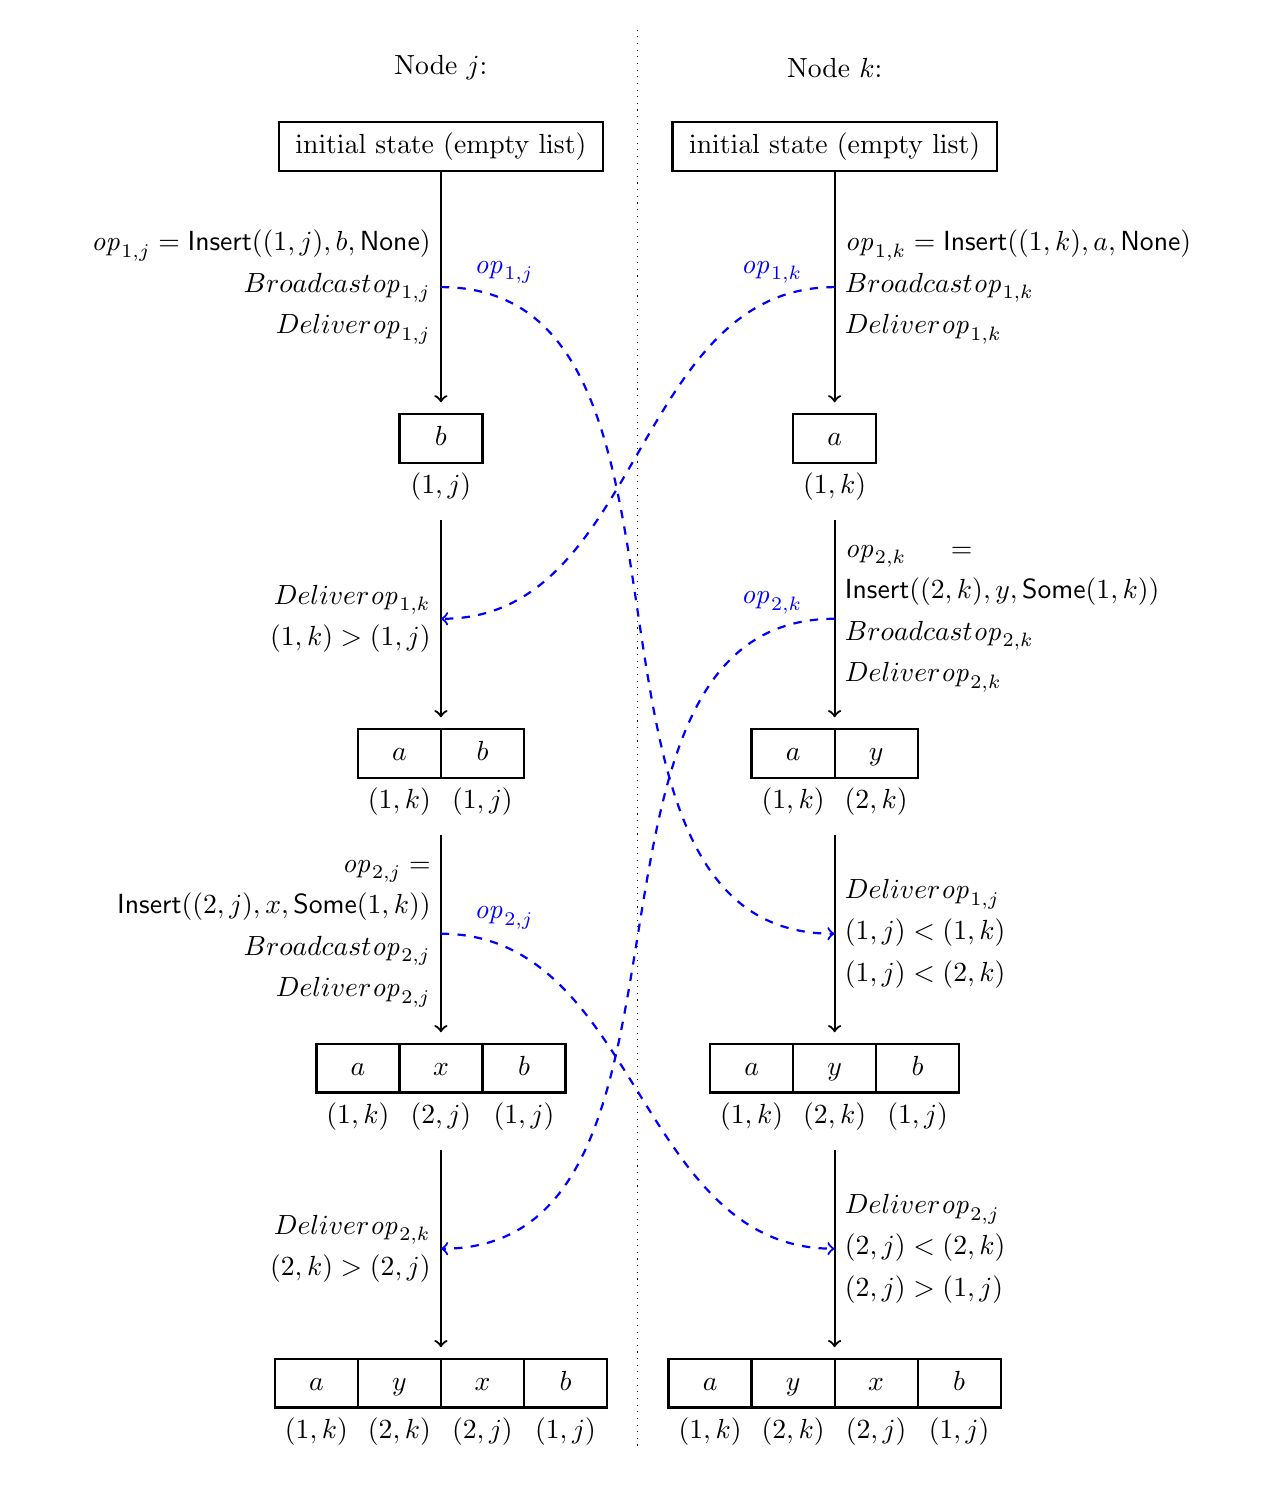
\begin{tikzpicture}[auto,scale=1.0]
\onehalfspacing
\path [draw,dotted] (2.5,-0.5) -- (2.5,17.5);

\tikzstyle{initstate}=[rectangle,draw,inner xsep=6pt,text height=8pt,text depth=3pt]
\tikzstyle{state}=[matrix,column sep={30pt,between origins}]
\tikzstyle{val}=[draw,anchor=base,minimum width=30pt,text height=8pt,text depth=3pt]
\tikzstyle{oid}=[anchor=base]
\tikzstyle{leftevent}=[left,text width=5cm,text ragged left,midway]
\tikzstyle{rightevent}=[right,text width=5cm,text ragged,midway]
\tikzstyle{every path}=[thick,->]

\node (leftR) at (0,17) {Node $j$:};
\node (left1) at (0,16) [initstate] {initial state (empty list)};
\node (left2) at (0,12) [state] {
    \node [val] {$b$};     \\
    \node [oid] {$(1,j)$}; \\
};
\node (left3) at (0,8) [state] {
    \node [val] {$a$};     & \node [val] {$b$};     \\
    \node [oid] {$(1,k)$}; & \node [oid] {$(1,j)$}; \\
};
\node (left4) at (0,4) [state] {
    \node [val] {$a$};     & \node [val] {$x$};     & \node [val] {$b$};     \\
    \node [oid] {$(1,k)$}; & \node [oid] {$(2,j)$}; & \node [oid] {$(1,j)$}; \\
};
\node (left5) at (0,0) [state] {
    \node [val] {$a$};     & \node [val] {$y$};     & \node [val] {$x$};     & \node [val] {$b$};     \\
    \node [oid] {$(1,k)$}; & \node [oid] {$(2,k)$}; & \node [oid] {$(2,j)$}; & \node [oid] {$(1,j)$}; \\
};

\draw (left1) -- (left2) node (send1j) [leftevent] {
    \hfill $\mathit{op}_{1,j} = \mathsf{Insert}((1, j), b, \mathsf{None})$ \\
    \hfill $\text{Broadcast } \mathit{op}_{1,j}$ \\
    \hfill $\text{Deliver } \mathit{op}_{1,j}$ \\
};
\draw (left2) -- (left3) node (recv1k) [leftevent] {
    \hfill $\text{Deliver } \mathit{op}_{1,k}$ \\
    \hfill $(1,k) > (1,j)$ \\
};
\draw (left3) -- (left4) node (send2j) [leftevent] {
    \hfill $\mathit{op}_{2,j} = \mathsf{Insert}((2, j), x, \mathsf{Some}(1,k))$ \\
    \hfill $\text{Broadcast } \mathit{op}_{2,j}$ \\
    \hfill $\text{Deliver } \mathit{op}_{2,j}$ \\
};
\draw (left4) -- (left5) node (recv2k) [leftevent] {
    \hfill $\text{Deliver } \mathit{op}_{2,k}$ \\
    \hfill $(2,k) > (2,j)$ \\
};

\node (rightR) at (5,17) {Node $k$:};
\node (right1) at (5,16) [initstate] {initial state (empty list)};
\node (right2) at (5,12) [state] {
    \node [val] {$a$};     \\
    \node [oid] {$(1,k)$}; \\
};
\node (right3) at (5,8) [state] {
    \node [val] {$a$};     & \node [val] {$y$};     \\
    \node [oid] {$(1,k)$}; & \node [oid] {$(2,k)$}; \\
};
\node (right4) at (5,4) [state] {
    \node [val] {$a$};     & \node [val] {$y$};     & \node [val] {$b$};     \\
    \node [oid] {$(1,k)$}; & \node [oid] {$(2,k)$}; & \node [oid] {$(1,j)$}; \\
};
\node (right5) at (5,0) [state] {
    \node [val] {$a$};     & \node [val] {$y$};     & \node [val] {$x$};     & \node [val] {$b$};     \\
    \node [oid] {$(1,k)$}; & \node [oid] {$(2,k)$}; & \node [oid] {$(2,j)$}; & \node [oid] {$(1,j)$}; \\
};

\draw (right1) -- (right2) node (send1k) [rightevent] {
    $\mathit{op}_{1,k} = \mathsf{Insert}((1, k), a, \mathsf{None})$ \\
    $\text{Broadcast } \mathit{op}_{1,k}$ \\
    $\text{Deliver } \mathit{op}_{1,k}$ \\
};
\draw (right2) -- (right3) node (send2k) [rightevent] {
    $\mathit{op}_{2,k} = \mathsf{Insert}((2, k), y, \mathsf{Some}(1, k))$ \\
    $\text{Broadcast } \mathit{op}_{2,k}$ \\
    $\text{Deliver } \mathit{op}_{2,k}$ \\
};
\draw (right3) -- (right4) node (recv1j) [rightevent] {
    $\text{Deliver } \mathit{op}_{1,j}$ \\
    $(1,j) < (1,k)$ \\
    $(1,j) < (2,k)$ \\
};
\draw (right4) -- (right5) node (recv2j) [rightevent] {
    $\text{Deliver } \mathit{op}_{2,j}$ \\
    $(2,j) < (2,k)$ \\
    $(2,j) > (1,j)$ \\
};

\begin{scope}[dashed,blue]
    \tikzstyle{every node}=[text centered]
    \draw (send1j.east) to [out=0,in=180] (recv1j.west);
    \draw (send2j.east) to [out=0,in=180] (recv2j.west);
    \draw (send1k.west) to [out=180,in=0] (recv1k.east);
    \draw (send2k.west) to [out=180,in=0] (recv2k.east);
    \node at (0.8,14.4) {$\mathit{op}_{1,j}$};
    \node at (0.8, 6.2) {$\mathit{op}_{2,j}$};
    \node at (4.2,14.4) {$\mathit{op}_{1,k}$};
    \node at (4.2,10.2) {$\mathit{op}_{2,k}$};
\end{scope}
\end{tikzpicture}

\caption{RGA example}\label{fig.two-lists}
\end{figure}


\subsection{An overview of Isabelle}
\label{subsect.an.overview.of.isabelle}

All of our proofs are checked with the Isabelle proof assistant~\cite{DBLP:conf/tphol/WenzelPN08}.
Accordingly, we now provide a brief introduction to the Isabelle logical framework and to the Isabelle/HOL object logic, so that the reader can easily follow our proofs and understand our theorem statements.
The interested reader is invited to reference standard tutorial material on Isabelle for a more in-depth introduction to the system~\cite{DBLP:books/sp/NipkowK14}.

Isabelle is a logical framework, providing a weak meta-logic---a fragment of intuitionistic higher-order logic---within which object logics may be embedded as theories.
One particular object logic embedding---Isabelle/HOL, a more expressive implementation of Gordon's higher-order logic~\cite{DBLP:conf/tphol/Gordon91} than that provided by the meta-logic---is the arena in which we formalise our proof of convergence.
Unlike systems based around Constructive Type Theory---such as Agda~\cite{DBLP:conf/tphol/BoveDN09}, Coq~\cite{DBLP:conf/popl/HuetH14}, or Matita~\cite{DBLP:conf/cade/AspertiRCT11}---Isabelle/HOL implements a classical logic.

Isabelle/HOL is a strictly-typed logic.
The logic's type system resembles that of mainstream functional programming languages, such as Standard ML, OCaml, or Haskell, albeit without the let-polymorphism that each of these languages implement.
\emph{Function types} are written $\tau_1 \Rightarrow \tau_2$, and are inhabited by \emph{total} functions, mapping elements of $\tau_1$ to elements of $\tau_2$.
Here, `total' means that all recursive function definitions must terminate i.e. recurse on some smaller argument, with respect to a well-founded order.
We write $\tau_1 \times \tau_2$ for the \emph{product type} of $\tau_1$ and $\tau_2$, inhabited by pairs of elements of type $\tau_1$ and $\tau_2$, respectively.
In a similar fashion to Standard ML and OCaml, but differing from Haskell, \emph{type operators} are applied to arguments in reverse order.
We therefore write $\tau\ \isa{list}$ and $\tau\ \isa{set}$ for the type of lists of elements of type $\tau$, and the type of mathematical (i.e. potentially infinite) sets of type $\tau$, respectively.
Type variable are written in lowercase, and preceded with a prime: ${\isacharprime}a \Rightarrow {\isacharprime}a$ denotes the type of a polymorphic identity function, for example.
\emph{Tagged union} types are introduced with the $\isacommand{datatype}$ keyword.
Constructors of tagged union types are written with an initial upper case letter.

In Isabelle/HOL's term language we write $\isa{t} \isa{::} \tau$ for a \emph{type ascription}, constraining the type of the term $\isa{t}$ to the type $\tau$.
We write $\lambda{x}. t$ for an anonymous function mapping an argument $\isa{x}$ to $\isa{t(x)}$, and write the application of term $\isa{t}$ with function type to an argument $\isa{u}$ as $\isa{t\ u}$, as usual.
Terms of list type are introduced using one of two constructors: $\isa{[]}$, or `nil', standing for the empty list, and infix $\isa{\#}$, or `cons', which prepends an element to an existing list.
We use $[t_1, \ldots, t_n]$ as syntactic sugar for a list literal, which is desugared into a series of cons applications.
We write $\{\}$ for the empty set, and use usual mathematical notation for set union, disjunction, membership tests, and so on: $\isa{t} \cup \isa{u}$, $\isa{t} \cap \isa{u}$, and $\isa{x} \in \isa{t}$.
Local definitions, within the body of a term, may be made with a let-in construct that is merely syntactic sugar for an unreduced $\beta$-redex.

Terms with type $\isa{bool}$ are called \emph{formulae}.
We write $\isa{True}$ and $\isa{False}$ for the logical truthity and falsity constants, respectively.
We write $\isa{t} \longrightarrow \isa{u}$, $\isa{t} \wedge \isa{u}$, and $\isa{t} \vee \isa{u}$ for material implication, conjunction, and disjunction, respectively, between formulae, and write $\neg t$ for the negation of a formula.
Isabelle/HOL's equality constant is polymorphic: we write $t = u$ for an assertion of equality between two terms of the same type.
We write $\forall{x}.t$ and $\exists{x}.t$ for universal and existential quantification---and write $\forall{x{\in}t}.u$ and $\exists{x{\in}t}.u$ for their bounded forms, restricted to members of a set $\isa{t}$.
An alternative implication arrow $\isa{t} \Longrightarrow \isa{u}$ may sometimes be used, and is in fact required by Isabelle in certain contexts.
The presence of this implication arrow is an artefact of Isabelle's status as a logical framework with object logics embedding into a meta-logic.
The reader may simply ignore this distinction between the `fat' and `thin' implication arrows as minor syntactic bureaucracy with no effect on their understanding.

New non-recursive definitions are entered into Isabelle's global context via the $\mathbf{definition}$ keyword.
Recursive functions are entered via the $\mathbf{fun}$ keyword, with functions being defined piecewise by pattern matching on inputs with a series of equations.
As mentioned, all recursive functions must be provably terminating, in that they recurse on arguments that are `smaller' with respect to a well-founded relation.
Most termination proofs are generated automatically by Isabelle itself, however, which has sophisticated automation dedicated to this task.

Inductive relations are used extensively in our formalisation, and are introduced with the $\mathbf{inductive}$ keyword.
An inductive relation definition of the form
\\
\begin{isabellebody}
\ \ \ \ \ \ \ \ \isacommand{inductive} foo\ {\isacharcolon}{\isacharcolon}\ {\isachardoublequoteopen}nat\ list\ {\isasymRightarrow}\ bool{\isachardoublequoteclose}\ \isakeyword{where}\isanewline
\ \ \ \ \ \ \ \ \ \ {\isachardoublequoteopen}foo\ {\isacharbrackleft}{\isacharbrackright}{\isachardoublequoteclose}\ {\isacharbar}\isanewline
\ \ \ \ \ \ \ \ \ \ {\isachardoublequoteopen}{\isasymlbrakk}\ foo\ xs\ {\isasymrbrakk}\ {\isasymLongrightarrow}\ foo {\isacharparenleft}5\#xs{\isacharparenright}{\isachardoublequoteclose}
\end{isabellebody}
\vspace{\baselineskip}
\noindent
introduces a new constant $\isa{foo}$ of type $\isa{nat list} \Rightarrow \isa{bool}$.
The two clauses in the body of the definition enumerate the conditions under which $\isa{foo}\ \isa{xs}$ is true, for arbitrary $\isa{xs}$.
The definition above states that $\isa{foo}$ is true at the empty list, or given a proof that $\isa{foo}\ \isa{xs}$ is true for some $\isa{xs}$, then $\isa{foo}\ (5\#\isa{xs})$ is true, also.
Further, $\isa{foo}\ \isa{xs}$ is true in no other circumstances, i.e. $\isa{foo}$ is the \emph{smallest} relation closed under the rules defining it.
In short, the clauses defining $\isa{foo}$ above state that $\isa{foo}\ \isa{xs}$ holds exactly in the case where $\isa{xs}$ is a (potentially empty) list containing only repeated copies of the natural number $5$.
Note that each clause above, and each clause in any inductive relation definition, can be interpreted as defining a series of inference rules, where assertions appearing to the left of $\Longrightarrow$ are understood as a rule's premisses, and assertions appearing to the right of the arrow are understood to be the rule's conclusion.
Clauses without an arrow can be interpreted as inference rules without premisses, or the `axioms' of the inductive relation definition.
Note that Isabelle will automatically generate custom induction, case analysis, and introduction theorems, tied to the definition of $\isa{foo}$, above, at the time of definition.

Lemmas, theorems, and corollaries can be asserted using the $\mathbf{lemma}$, $\mathbf{theorem}$, and $\mathbf{corollary}$ keywords, respectively.
There is no semantic difference between these keywords in Isabelle---any relative import between a lemma statement and a theorem statement is purely in the eye of the beholder.
A theorem statement of the form
\\
\begin{isabellebody}
\ \ \ \ \ \ \ \ \isacommand{theorem} goo{\isacharcolon}\isanewline
\ \ \ \ \ \ \ \ \ \ \isakeyword{assumes}\ foo\ xs \isakeyword{and}\ foo\ ys \isanewline
\ \ \ \ \ \ \ \ \ \ \isakeyword{shows}\ foo (xs \isacharat ys)
\end{isabellebody}
\vspace{\baselineskip}
\noindent
produces a proof obligation, wherein the user is tasked with proving $\isa{foo} (xs \isacharat ys)$ under the two assumptions $\isa{foo}\ xs$ and $\isa{foo}\ ys$, where $xs \isacharat ys$ denotes the appending of two lists $\isa{xs}$ and $\isa{ys}$.
An optional name, here $\isa{goo}$, is assigned to the theorem, so that it may be referenced in later proofs.

Closing a proof obligation can proceed in one of two ways in Isabelle/HOL.
`Apply-style' tactic driven theorem proving is one method, which sees a proof obligation decomposed into simpler subgoals in a backwards-directed manner, using \emph{tactics}---small programs that aim to progress a backwards proof by decomposing, or solving outright, a proof obligation.
An alternative style uses the Isar structured proof language~\cite{DBLP:phd/dnb/Wenzel02a}, which attempts to mimic the structure and form of human-written proofs in a completely machine-checked way, and is claimed to be closer to informal mathematical practice than the alternative `apply-style' proofs.
We use both styles of proof in this formalisation, depending on the particular theorem and its relative importance.

Lastly, we use \emph{locales}---or local theory environments~\cite{DBLP:conf/tphol/KammullerWP99,DBLP:conf/types/HaftmannW08}---extensively throughout our development to structure the proof.
A declaration of the form
\\
\begin{isabellebody}
\ \ \ \ \ \ \ \ \isacommand{locale} hoo = \isanewline
\ \ \ \ \ \ \ \ \ \ \isakeyword{fixes}\ f\ {\isacharcolon}{\isacharcolon}\ {\isachardoublequoteopen}{\isacharprime}a\ {\isasymRightarrow}\ {\isacharprime}a{\isachardoublequoteclose}\isanewline
\ \ \ \ \ \ \ \ \ \ \isakeyword{assumes} {\isachardoublequoteopen}f\ x = x{\isachardoublequoteclose}
\end{isabellebody}
\vspace{\baselineskip}
\noindent
introduces a local theory, with a fixed, typed constant $\isa{f}$, and an associated law that states that $\isa{f}$ is the identity function.
Functions and constants may now be defined, and theorems conjectured and proved, within the context of the $\isa{hoo}$ theory---this is indicated syntactically by writing $(\isacommand{in}\ hoo)$ before the name of the constant being defined, or the theorem being conjectured, at the point of definition or conjecture.
Any function, constant, or theorem, marked in this way may make reference to $\isa{f}$, or the fact that $\isa{f}\ \isa{x} = \isa{x}$ for all $\isa{x}$.
\emph{Interpreting} a local theory---such as $\isa{hoo}$ above---involves providing a concrete implementation of $\isa{f}$ coupled with a proof that the concrete implementation satisfies the associated law.
Once interpreted, all functions, definitions, and theorems made within the $\isa{hoo}$ local theory become available to use for that concrete implementation.

\section{High-level proof strategy}
\label{sect.high-level.proof.strategy}

Before embarking on a detailed description of our formal proof of convergence in Isabelle, we provide a higher-level overview of the proof strategy used.

%%%%%%%%%%%%%%%%%%%%%%%%%%%%%%%%%%%%%%%%%%%%%%%%%%%%%%%%%%%%%%%%%%%%%%%%%%%%%%%%
% Convergence
%%%%%%%%%%%%%%%%%%%%%%%%%%%%%%%%%%%%%%%%%%%%%%%%%%%%%%%%%%%%%%%%%%%%%%%%%%%%%%%%

\section{Convergence}
\label{sect.convergence}

\subsection{Our consistency model, and main theorem statement}
\label{subsect.consistency.model.main.theorem.statement}

\emph{Strong eventual consistency} is a special case of eventual consistency.
In a strongly eventual consistent system, the operations that a replica may use to modify subcomponents of the system's shared global state are constrained in such a way that pairs of operations naturally commute with each other.
As a result, the system will eventually reach a consistent state, but the potentially error prone process of invoking conflict resolution strategies is no longer needed, as conflicts are impossible to introduce, by construction.
This consistency model is impossible to achieve for many distributed systems, but it is the natural consistency model---and therefore notion of correctness---for Conflict-free Replicated Datatypes, whose operations are guaranteed to commute, as previously described.

In this work, we prove that our Replicated Growable Array implementation possesses this convergence property in an abstract setting.
Our final theorem states that two arbitrary lists of distinct events enriched by an order relation, that satisfy a consistency property defined in terms of a \emph{happens before} relation, converge to the same state.
Formally, we prove:
\\
\begin{isabellebody}
\ \ \ \ \isacommand{theorem} convergence{\isacharcolon}\isanewline
\ \ \ \ \ \ \isakeyword{assumes}\ {\isachardoublequoteopen}set\ xs\ {\isacharequal}\ set\ ys{\isachardoublequoteclose}\isanewline
\ \ \ \ \ \ \ \ \ \ \isakeyword{and}\ {\isachardoublequoteopen}concurrent{\isacharunderscore}ops{\isacharunderscore}commute\ xs{\isachardoublequoteclose}\ \isakeyword{and}\ {\isachardoublequoteopen}concurrent{\isacharunderscore}ops{\isacharunderscore}commute\ ys{\isachardoublequoteclose}\isanewline
\ \ \ \ \ \ \ \ \ \ \isakeyword{and}\ {\isachardoublequoteopen}distinct\ xs{\isachardoublequoteclose}\ \isakeyword{and}\ {\isachardoublequoteopen}distinct\ ys{\isachardoublequoteclose}\isanewline
\ \ \ \ \ \ \ \ \ \ \isakeyword{and}\ {\isachardoublequoteopen}hb{\isacharunderscore}consistent\ xs{\isachardoublequoteclose}\ \isakeyword{and}\ {\isachardoublequoteopen}hb{\isacharunderscore}consistent\ ys{\isachardoublequoteclose}\isanewline
\ \ \ \ \ \ \ \ \isakeyword{shows}\ {\isachardoublequoteopen}apply{\isacharunderscore}operations\ xs\ {\isacharequal}\ apply{\isacharunderscore}operations\ ys{\isachardoublequoteclose}\isanewline
\end{isabellebody}
That is, suppose $\isa{xs}$ and $\isa{ys}$ are two arbitrary list of distinct events, that contain the same set of elements, but are ordered in a way that respects our \emph{happens before} relation---that is, so earlier elements in the list all \emph{happen before} later ones.
Suppose also that any two events in $\isa{xs}$ (respectively, $\isa{ys}$) that happen concurrently, per our \emph{happens before} relation, have a commuting property on states.
Then the final state one obtains by applying

Let $\mathit{Events}$ be the set of events enriched with a preorder $\prec$. We
write $\isa{x} \prec \isa{y}$ and say that the event \isa{x} \emph{happens
before} the event \isa{y}.  Moreover we assume that there exists an
interpretation partial function $\langle\_\rangle$ that maps events to
\emph{operations}, which are \emph{state transformers} on a set of states
$\Sigma$.  This is implemented in Isabelle by the following locale
statement.

\begin{isabellebody}
  \isanewline
\isacommand{locale}\isamarkupfalse%
\ happens{\isacharunderscore}before\ {\isacharequal}\ preorder\ hb{\isacharunderscore}weak\ hb\isanewline
\ \ \isakeyword{for}\ hb{\isacharunderscore}weak\ {\isacharcolon}{\isacharcolon}\ {\isachardoublequoteopen}{\isacharprime}a\ {\isasymRightarrow}\ {\isacharprime}a\ {\isasymRightarrow}\ bool{\isachardoublequoteclose}\ \ {\isacharparenleft}\isakeyword{infix}\ {\isachardoublequoteopen}{\isasympreceq}{\isachardoublequoteclose}\ {\isadigit{5}}{\isadigit{0}}{\isacharparenright}\isanewline
\ \ \isakeyword{and}\ hb\ {\isacharcolon}{\isacharcolon}\ {\isachardoublequoteopen}{\isacharprime}a\ {\isasymRightarrow}\ {\isacharprime}a\ {\isasymRightarrow}\ bool{\isachardoublequoteclose}\ \ \ \ \ \ \ {\isacharparenleft}\isakeyword{infix}\ {\isachardoublequoteopen}{\isasymprec}{\isachardoublequoteclose}\ {\isadigit{5}}{\isadigit{0}}{\isacharparenright}\ {\isacharplus}\isanewline
\ \ \isakeyword{fixes}\ interp\ {\isacharcolon}{\isacharcolon}\ {\isachardoublequoteopen}{\isacharprime}a\ {\isasymRightarrow}\ {\isacharprime}b\ {\isasymrightharpoonup}\ {\isacharprime}b{\isachardoublequoteclose}\ {\isacharparenleft}{\isachardoublequoteopen}{\isasymlangle}{\isacharunderscore}{\isasymrangle}{\isachardoublequoteclose}\ {\isacharbrackleft}{\isadigit{0}}{\isacharbrackright}\ {\isadigit{1}}{\isadigit{0}}{\isadigit{0}}{\isadigit{0}}{\isacharparenright}\isanewline
\end{isabellebody}

We say that two events (or operations) $x$ and $y$ are \emph{concurrent}
whenever one does not happens before the other, that is, $\neg (\isa{x} \prec
\isa{y})$ and $\neg (\isa{y} \prec \isa{x})$.

\begin{isabellebody}
  \isanewline
\isacommand{definition}\isamarkupfalse%
\ concurrent\ {\isacharcolon}{\isacharcolon}\ {\isachardoublequoteopen}{\isacharprime}a\ {\isasymRightarrow}\ {\isacharprime}a\ {\isasymRightarrow}\ bool{\isachardoublequoteclose}\ {\isacharparenleft}\isakeyword{infix}\ {\isachardoublequoteopen}{\isasymparallel}{\isachardoublequoteclose}\ {\isadigit{5}}{\isadigit{0}}{\isacharparenright}\ \isakeyword{where}\isanewline
\ \ {\isachardoublequoteopen}x\ {\isasymparallel}\ y\ {\isasymequiv}\ {\isasymnot}\ {\isacharparenleft}x\ {\isasymprec}\ y{\isacharparenright}\ {\isasymand}\ {\isasymnot}\ {\isacharparenleft}y\ {\isasymprec}\ x{\isacharparenright}{\isachardoublequoteclose}\isanewline
\end{isabellebody}

A list of events \isa{xs} is \emph{hb-consistent}, or simply \emph{consistent},
whenever for any element \isa{y}, it is not the case that \isa{y} happens
before \isa{x} for all \isa{x} that appears before \isa{y} in the list. That
is, \isa{x} and \isa{y} are either concurrent or \isa{x} happens before
\isa{y}.  This is implemented in Isabelle by an inductive predicate.

\begin{isabellebody}
  \isanewline
\isacommand{inductive}\isamarkupfalse%
\ hb{\isacharunderscore}consistent\ {\isacharcolon}{\isacharcolon}\ {\isachardoublequoteopen}{\isacharprime}a\ list\ {\isasymRightarrow}\ bool{\isachardoublequoteclose}\ \isakeyword{where}\isanewline
\ \ {\isachardoublequoteopen}hb{\isacharunderscore}consistent\ {\isacharbrackleft}{\isacharbrackright}{\isachardoublequoteclose}\ {\isacharbar}\isanewline
\ \ {\isachardoublequoteopen}{\isasymlbrakk}\ hb{\isacharunderscore}consistent\ xs{\isacharsemicolon}\ {\isasymforall}x\ {\isasymin}\ set\ xs{\isachardot}\ {\isasymnot}\ y\ {\isasymprec}\ x\ {\isasymrbrakk}\ {\isasymLongrightarrow}\ hb{\isacharunderscore}consistent\ {\isacharparenleft}xs\ {\isacharat}\ {\isacharbrackleft}y{\isacharbrackright}{\isacharparenright}{\isachardoublequoteclose}\isanewline
\end{isabellebody}

Additionally, we say that concurrent operations commute in a list \isa{xs}
whenever for all concurrent events \isa{x} and \isa{y} in the list \isa{xs},
the Kleisli arrow composition of their operations commute $\langle \isa{x}
\rangle \rhd \langle \isa{y} \rangle = \langle \isa{y} \rangle \rhd \langle
\isa{x} \rangle$.

\begin{isabellebody}
  \isanewline
\isacommand{definition}\isamarkupfalse%
\ concurrent{\isacharunderscore}ops{\isacharunderscore}commute\ {\isacharcolon}{\isacharcolon}\ {\isachardoublequoteopen}{\isacharprime}a\ list\ {\isasymRightarrow}\ bool{\isachardoublequoteclose}\ \isakeyword{where}\isanewline
\ \ {\isachardoublequoteopen}concurrent{\isacharunderscore}ops{\isacharunderscore}commute\ xs\ {\isasymequiv}
\ {\isasymforall}x\ y{\isachardot}\ {\isacharbraceleft}x{\isacharcomma}\ y{\isacharbraceright}\ {\isasymsubseteq}\ set\ xs\ {\isasymlongrightarrow}\ x\ {\isasymparallel}\ y\ {\isasymlongrightarrow}\ {\isasymlangle}x{\isasymrangle}{\isasymrhd}{\isasymlangle}y{\isasymrangle}\ {\isacharequal}\ {\isasymlangle}y{\isasymrangle}{\isasymrhd}{\isasymlangle}x{\isasymrangle}{\isachardoublequoteclose}\isanewline

\isacommand{definition}\isamarkupfalse%
\ kleisli\ {\isacharcolon}{\isacharcolon}\ {\isachardoublequoteopen}{\isacharparenleft}{\isacharprime}b\ {\isasymRightarrow}\ {\isacharprime}b\ option{\isacharparenright}\ {\isasymRightarrow}\ {\isacharparenleft}{\isacharprime}b\ {\isasymRightarrow}\ {\isacharprime}b\ option{\isacharparenright}\ {\isasymRightarrow}\ {\isacharparenleft}{\isacharprime}b\ {\isasymRightarrow}\ {\isacharprime}b\ option{\isacharparenright}{\isachardoublequoteclose}\ {\isacharparenleft}\isakeyword{infixr}\ {\isachardoublequoteopen}{\isasymrhd}{\isachardoublequoteclose}\ {\isadigit{6}}{\isadigit{5}}{\isacharparenright}\ \isakeyword{where}\isanewline
\ \ {\isachardoublequoteopen}f\ {\isasymrhd}\ g\ {\isasymequiv}\ {\isasymlambda}x{\isachardot}\ f\ x\ {\isasymbind}\ {\isacharparenleft}{\isasymlambda}fx{\isachardot}\ g\ fx{\isacharparenright}{\isachardoublequoteclose}\isanewline
\end{isabellebody}

Let \isa{xs} be a list of events, \isa{apply-operations\ xs} is the state
transformer equivalent of applying in order each operation $\langle \isa{x}
\rangle$ for events \isa{x} in the list.  In other words, it is the fold of
the Kleisli arrow composition on the associated list of operations.

\begin{isabellebody}
  \isanewline
\isacommand{definition}\isamarkupfalse%
\ apply{\isacharunderscore}operations\ {\isacharcolon}{\isacharcolon}\ {\isachardoublequoteopen}{\isacharprime}a\ list\ {\isasymRightarrow}\ {\isacharprime}b\ {\isasymrightharpoonup}\ {\isacharprime}b{\isachardoublequoteclose}\ \isakeyword{where}\isanewline
\ \ {\isachardoublequoteopen}apply{\isacharunderscore}operations\ es\ s\ {\isasymequiv}\ {\isacharparenleft}foldl\ {\isacharparenleft}op\ {\isasymrhd}{\isacharparenright}\ Some\ {\isacharparenleft}map\ interp\ es{\isacharparenright}{\isacharparenright}\ s{\isachardoublequoteclose}\isanewline
\end{isabellebody}

\begin{isabellebody}
\isacommand{lemma}\isamarkupfalse%
\ concurrent{\isacharunderscore}ops{\isacharunderscore}commute{\isacharunderscore}concurrent{\isacharunderscore}set{\isacharcolon}\isanewline
\ \ \isakeyword{assumes}\ {\isachardoublequoteopen}concurrent{\isacharunderscore}ops{\isacharunderscore}commute\ {\isacharparenleft}prefix{\isacharat}suffix{\isacharat}{\isacharbrackleft}x{\isacharbrackright}{\isacharparenright}{\isachardoublequoteclose}\isanewline
\ \ \ \ \ \ \ \ \ \ {\isachardoublequoteopen}concurrent{\isacharunderscore}set\ x\ suffix{\isachardoublequoteclose}\isanewline
\ \ \ \ \ \ \ \ \ \ {\isachardoublequoteopen}distinct\ {\isacharparenleft}prefix\ {\isacharat}\ x\ {\isacharhash}\ suffix{\isacharparenright}{\isachardoublequoteclose}\isanewline
\ \ \isakeyword{shows}\ \ \ {\isachardoublequoteopen}apply{\isacharunderscore}operations\ {\isacharparenleft}prefix\ {\isacharat}\ suffix\ {\isacharat}\ {\isacharbrackleft}x{\isacharbrackright}{\isacharparenright}\ {\isacharequal}\ apply{\isacharunderscore}operations\ {\isacharparenleft}prefix\ {\isacharat}\ x\ {\isacharhash}\ suffix{\isacharparenright}{\isachardoublequoteclose}\isanewline
\end{isabellebody}

We can now formally state the abstract convergence theorem: two consistent list
of distinct events in which concurrent operations commute that have the same
set of elements yield the same state transformer.

\begin{isabellebody}
  \isanewline
\isacommand{theorem}\isamarkupfalse%
\ \ convergence{\isacharcolon}\isanewline
\ \ \isakeyword{assumes}\ {\isachardoublequoteopen}set\ xs\ {\isacharequal}\ set\ ys{\isachardoublequoteclose}\isanewline
\ \ \ \ \ \ \ \ \ \ {\isachardoublequoteopen}concurrent{\isacharunderscore}ops{\isacharunderscore}commute\ xs{\isachardoublequoteclose}\isanewline
\ \ \ \ \ \ \ \ \ \ {\isachardoublequoteopen}concurrent{\isacharunderscore}ops{\isacharunderscore}commute\ ys{\isachardoublequoteclose}\isanewline
\ \ \ \ \ \ \ \ \ \ {\isachardoublequoteopen}distinct\ xs{\isachardoublequoteclose}\isanewline
\ \ \ \ \ \ \ \ \ \ {\isachardoublequoteopen}distinct\ ys{\isachardoublequoteclose}\isanewline
\ \ \ \ \ \ \ \ \ \ {\isachardoublequoteopen}hb{\isacharunderscore}consistent\ xs{\isachardoublequoteclose}\isanewline
\ \ \ \ \ \ \ \ \ \ {\isachardoublequoteopen}hb{\isacharunderscore}consistent\ ys{\isachardoublequoteclose}\isanewline
\ \ \isakeyword{shows}\ \ \ {\isachardoublequoteopen}apply{\isacharunderscore}operations\ xs\ {\isacharequal}\ apply{\isacharunderscore}operations\ ys{\isachardoublequoteclose}\isanewline
\end{isabellebody}

The entire proof is shown in Figure~\ref{fig.convergence}.  The proof follows
by induction on \isa{xs}. The empty list case is immediate. Assuming the
property for \isa{xs}, we prove the case when a new event \isa{x} is added to
the end of \isa{xs}, that is, $\isa{xs}@[\isa{x}]$. Since both lists have the
same elements, one can split \isa{ys} such that \isa{ys = prefix@x@suffix} for
some suitable lists \isa{prefix} and \isa{suffix}. Moreover, all the events in
the set of \isa{suffix} is concurrent to \isa{x}. By the induction hypothesis,
\isa{apply-operations\ xs $=$ apply-operations\ (prefix $@$ suffix)}. Then
\begin{align*}
  \isa{apply-operations}\ (\isa{xs}@[\isa{x}])
  &= \langle\isa{x}\rangle\ (\isa{apply-operations}\ \isa{xs}) \\
  &= \langle\isa{x}\rangle\ (\isa{apply-operations}\ (\isa{prefix}@\isa{suffix}))\\
  &= \isa{apply-operations} (\isa{prefix}@\isa{suffix}@\isa{x}) \\
  &= \isa{apply-operations} (\isa{prefix}@\isa{x@\isa{suffix}}) \\
  &= \isa{apply-operations}\ ys.
\end{align*}


\begin{figure}[t]
  \raggedright
  \begin{isabellebody}
\isanewline
\isacommand{theorem}\isamarkupfalse%
\ \ convergence{\isacharcolon}\isanewline
\ \ \isakeyword{assumes}\ {\isachardoublequoteopen}set\ xs\ {\isacharequal}\ set\ ys{\isachardoublequoteclose}\isanewline
\ \ \ \ \ \ \ \ \ \ {\isachardoublequoteopen}concurrent{\isacharunderscore}ops{\isacharunderscore}commute\ xs{\isachardoublequoteclose}\isanewline
\ \ \ \ \ \ \ \ \ \ {\isachardoublequoteopen}concurrent{\isacharunderscore}ops{\isacharunderscore}commute\ ys{\isachardoublequoteclose}\isanewline
\ \ \ \ \ \ \ \ \ \ {\isachardoublequoteopen}distinct\ xs{\isachardoublequoteclose}\isanewline
\ \ \ \ \ \ \ \ \ \ {\isachardoublequoteopen}distinct\ ys{\isachardoublequoteclose}\isanewline
\ \ \ \ \ \ \ \ \ \ {\isachardoublequoteopen}hb{\isacharunderscore}consistent\ xs{\isachardoublequoteclose}\isanewline
\ \ \ \ \ \ \ \ \ \ {\isachardoublequoteopen}hb{\isacharunderscore}consistent\ ys{\isachardoublequoteclose}\isanewline
\ \ \isakeyword{shows}\ \ \ {\isachardoublequoteopen}apply{\isacharunderscore}operations\ xs\ {\isacharequal}\ apply{\isacharunderscore}operations\ ys{\isachardoublequoteclose}\isanewline
%
\isacommand{using}\isamarkupfalse%
\ assms\ \isacommand{proof}\isamarkupfalse%
{\isacharparenleft}induction\ xs\ arbitrary{\isacharcolon}\ ys\ rule{\isacharcolon}\ rev{\isacharunderscore}induct{\isacharcomma}\ simp{\isacharparenright}\isanewline
\ \ \isacommand{case}\isamarkupfalse%
\ assms{\isacharcolon}\ {\isacharparenleft}snoc\ x\ xs{\isacharparenright}\isanewline
\ \ \isacommand{then}\isamarkupfalse%
\ \isacommand{obtain}\isamarkupfalse%
\ prefix\ suffix\ \isakeyword{where}\ ys{\isacharunderscore}split{\isacharcolon}\ {\isachardoublequoteopen}ys\ {\isacharequal}\ prefix\ {\isacharat}\ x\ {\isacharhash}\ suffix\ {\isasymand}\ concurrent{\isacharunderscore}set\ x\ suffix{\isachardoublequoteclose}\isanewline
\ \ \ \ \isacommand{using}\isamarkupfalse%
\ hb{\isacharunderscore}consistent{\isacharunderscore}prefix{\isacharunderscore}suffix{\isacharunderscore}exists\ \isacommand{by}\isamarkupfalse%
\ fastforce\isanewline
\ \ \isacommand{moreover}\isamarkupfalse%
\ \isacommand{hence}\isamarkupfalse%
\ {\isacharasterisk}{\isacharcolon}\ {\isachardoublequoteopen}distinct\ {\isacharparenleft}prefix\ {\isacharat}\ suffix{\isacharparenright}{\isachardoublequoteclose}\ {\isachardoublequoteopen}hb{\isacharunderscore}consistent\ xs{\isachardoublequoteclose}\isanewline
\ \ \ \ \isacommand{using}\isamarkupfalse%
\ assms\ \isacommand{by}\isamarkupfalse%
\ auto\isanewline
\ \ \isacommand{moreover}\isamarkupfalse%
\ \isacommand{{\isacharbraceleft}}\isamarkupfalse%
\isanewline
\ \ \ \ \isacommand{have}\isamarkupfalse%
\ {\isachardoublequoteopen}hb{\isacharunderscore}consistent\ prefix{\isachardoublequoteclose}\ {\isachardoublequoteopen}hb{\isacharunderscore}consistent\ suffix{\isachardoublequoteclose}\isanewline
\ \ \ \ \ \ \isacommand{using}\isamarkupfalse%
\ ys{\isacharunderscore}split\ assms\ hb{\isacharunderscore}consistent{\isacharunderscore}append{\isacharunderscore}D{\isadigit{2}}\ hb{\isacharunderscore}consistent{\isacharunderscore}append{\isacharunderscore}elim{\isacharunderscore}ConsD\ \isacommand{by}\isamarkupfalse%
\ blast{\isacharplus}\isanewline
\ \ \ \ \isacommand{hence}\isamarkupfalse%
\ {\isachardoublequoteopen}hb{\isacharunderscore}consistent\ {\isacharparenleft}prefix\ {\isacharat}\ suffix{\isacharparenright}{\isachardoublequoteclose}\isanewline
\ \ \ \ \ \ \isacommand{by}\isamarkupfalse%
\ {\isacharparenleft}metis\ assms{\isacharparenleft}{\isadigit{8}}{\isacharparenright}\ hb{\isacharunderscore}consistent{\isacharunderscore}append\ hb{\isacharunderscore}consistent{\isacharunderscore}append{\isacharunderscore}porder\ list{\isachardot}set{\isacharunderscore}intros{\isacharparenleft}{\isadigit{2}}{\isacharparenright}\ ys{\isacharunderscore}split{\isacharparenright}\isanewline
\ \ \isacommand{{\isacharbraceright}}\isamarkupfalse%
\isanewline
\ \ \isacommand{moreover}\isamarkupfalse%
\ \isacommand{have}\isamarkupfalse%
\ {\isacharasterisk}{\isacharasterisk}{\isacharcolon}\ {\isachardoublequoteopen}concurrent{\isacharunderscore}ops{\isacharunderscore}commute\ {\isacharparenleft}prefix\ {\isacharat}\ suffix\ {\isacharat}\ {\isacharbrackleft}x{\isacharbrackright}{\isacharparenright}{\isachardoublequoteclose}\isanewline
\ \ \ \ \isacommand{using}\isamarkupfalse%
\ assms\ ys{\isacharunderscore}split\ \isacommand{by}\isamarkupfalse%
\ {\isacharparenleft}clarsimp\ simp{\isacharcolon}\ concurrent{\isacharunderscore}ops{\isacharunderscore}commute{\isacharunderscore}def{\isacharparenright}\isanewline
\ \ \isacommand{moreover}\isamarkupfalse%
\ \isacommand{hence}\isamarkupfalse%
\ {\isachardoublequoteopen}concurrent{\isacharunderscore}ops{\isacharunderscore}commute\ {\isacharparenleft}prefix\ {\isacharat}\ suffix{\isacharparenright}{\isachardoublequoteclose}\isanewline
\ \ \ \ \isacommand{by}\isamarkupfalse%
\ {\isacharparenleft}force\ simp\ del{\isacharcolon}\ append{\isacharunderscore}assoc\ simp\ add{\isacharcolon}\ append{\isacharunderscore}assoc{\isacharbrackleft}symmetric{\isacharbrackright}{\isacharparenright}\isanewline
\ \ \isacommand{ultimately}\isamarkupfalse%
\ \isacommand{have}\isamarkupfalse%
\ {\isachardoublequoteopen}apply{\isacharunderscore}operations\ xs\ {\isacharequal}\ apply{\isacharunderscore}operations\ {\isacharparenleft}prefix{\isacharat}suffix{\isacharparenright}{\isachardoublequoteclose}\isanewline
\ \ \ \ \isacommand{using}\isamarkupfalse%
\ assms\ \isacommand{by}\isamarkupfalse%
\ simp\ {\isacharparenleft}metis\ Diff{\isacharunderscore}insert{\isacharunderscore}absorb\ Un{\isacharunderscore}iff\ {\isacharasterisk}\ concurrent{\isacharunderscore}ops{\isacharunderscore}commute{\isacharunderscore}appendD\ set{\isacharunderscore}append{\isacharparenright}\isanewline
\ \ \isacommand{moreover}\isamarkupfalse%
\ \isacommand{have}\isamarkupfalse%
\ {\isachardoublequoteopen}apply{\isacharunderscore}operations\ {\isacharparenleft}prefix{\isacharat}suffix\ {\isacharat}\ {\isacharbrackleft}x{\isacharbrackright}{\isacharparenright}\ {\isacharequal}\ apply{\isacharunderscore}operations\ {\isacharparenleft}prefix{\isacharat}x\ {\isacharhash}\ suffix{\isacharparenright}{\isachardoublequoteclose}\isanewline
\ \ \ \ \isacommand{using}\isamarkupfalse%
\ ys{\isacharunderscore}split\ assms\ {\isacharasterisk}{\isacharasterisk}\ concurrent{\isacharunderscore}ops{\isacharunderscore}commute{\isacharunderscore}concurrent{\isacharunderscore}set\ \isacommand{by}\isamarkupfalse%
\ force\isanewline
\ \ \isacommand{ultimately}\isamarkupfalse%
\ \isacommand{show}\isamarkupfalse%
\ {\isacharquery}case\isanewline
\ \ \ \ \isacommand{using}\isamarkupfalse%
\ ys{\isacharunderscore}split\ \isacommand{by}\isamarkupfalse%
\ {\isacharparenleft}force\ simp{\isacharcolon}\ append{\isacharunderscore}assoc{\isacharbrackleft}symmetric{\isacharbrackright}\ simp\ del{\isacharcolon}\ append{\isacharunderscore}assoc{\isacharparenright}\isanewline
\isacommand{qed}\isamarkupfalse%
  \end{isabellebody}
  \caption{Proof of convergence theorem in Isar.}
  \label{fig.convergence}
\end{figure}


%%%%%%%%%%%%%%%%%%%%%%%%%%%%%%%%%%%%%%%%%%%%%%%%%%%%%%%%%%%%%%%%%%%%%%%%%%%%%%%%
% Network
%%%%%%%%%%%%%%%%%%%%%%%%%%%%%%%%%%%%%%%%%%%%%%%%%%%%%%%%%%%%%%%%%%%%%%%%%%%%%%%%

\section{Network}
\label{sect.network}

In this section, we incrementally work towards a definition of an asynchronous causal network, considering a number of intermediary abstractions, and important definitions made using those abstractions, along the way.
We conclude the section by demonstrating that our convergence theorem---$\isa{convergence}$, discussed in the previous section---can be `lowered' into an asynchronous causal network, to obtain another convergence theorem.

We first consider a setting characterised by an arbitrary (unbounded) number of `nodes', `replicas', or `processes'.
Precisely what these nodes are, and what their pattern of communication is, if any, is left abstract at this point.
Aside from being unbounded in number, nodes in this setting have two key properties:
\begin{enumerate}
\item
They are uniquely named, and we can always refer to a node with some known unique identifier.
In our setting, we will identify the set of node identifiers with the set of natural numbers.
\item
Each node has an ordered finite history of abstract `events' associated with it---though, at this point we do not specify what these events actually are.
All that can be said is that this history is a `local' history, in that it details a series of network events as the particular node in question perceives them, not a `global' history of all network events seen by some external monitor.
We therefore insist that a node's history is not merely ordered, but has a strict total order structure imposed on it.
Further, every event in a node's history is assumed to be unique.
Uniqueness is a reasonable assumption, as we may use timestamps, globally unique identifiers, or some other disambiguation device attached to concrete messages to ensure that this property holds.
\end{enumerate}
We model the configuration of nodes described above with a local theory in Isabelle, which we call $\isa{node{\isacharunderscore}histories}$:
\\
\begin{isabellebody}
\ \ \ \ \ \ \ \ \isacommand{locale} node{\isacharunderscore}histories\ {\isacharequal}\ \isanewline
\ \ \ \ \ \ \ \ \ \ \isakeyword{fixes}\ history\ {\isacharcolon}{\isacharcolon}\ {\isachardoublequoteopen}nat\ {\isasymRightarrow}\ {\isacharprime}a\ list{\isachardoublequoteclose}\isanewline
\ \ \ \ \ \ \ \ \ \ \isakeyword{assumes}\ histories{\isacharunderscore}distinct{\isacharcolon}\ {\isachardoublequoteopen}distinct\ {\isacharparenleft}history\ i{\isacharparenright}{\isachardoublequoteclose}
\end{isabellebody}
\vspace{\baselineskip}
Here, the history of a node $\isa{i}$ is obtained by using a function fixed by the local theory, $\isa{history}$.
Concretely, we capture the fact that a node's local history is totally ordered by implementing histories as a list of events.
Events are simply modelled as a type variable---here we use $\isa{{\isacharprime}a}$---to ensure that they are completely abstract, with no internal structure.
The $\isa{distinct}$ predicate is an Isabelle/HOL library function which asserts that a list has no repeated elements, upto equality.

Note that the $\isa{node{\isacharunderscore}histories}$ locale is quite general: it can handle both a bounded and unbounded number of nodes.
In the former case, we simply assume that $\isa{history}$ is \emph{finitely supported}, in the sense that all but a bounded number of node histories are `empty', i.e. the function returns the empty list of events at those nodes.

Isabelle lists are finite, and therefore so is a node's history.
As a result, at the end of a node's history, we assume that a node has either \emph{failed} or successfully terminated.
In our model, a node can fail only once, which is modeled by the absence of any further events in the history, and after that it is deemed to have disconnected permanently from the network.
This \emph{crash-stop} abstraction is commonly used by distributed algorithms \cite{Cachin:2011wt}.
Crashes of one node cannot be detected by other nodes: a lack of messages at any given moment might indicate the crash of the sender, message loss, or network delay, and recipients of messages cannot distinguish between these causes.

In the general setting of the $\isa{node{\isacharunderscore}histories}$ local theory, we may define when one event comes before another, at a fixed node.
Writing $\isa{x} \sqsubset^\isa{i} \isa{y}$ for the \emph{comes before} relation at node $\isa{i}$, we assert that this relation holds whenever lists $\isa{xs}$, $\isa{ys}$ and $\isa{zs}$ exist such that $\isa{xs}@[\isa{x}]@\isa{ys}@[\isa{y}]@\isa{zs} = \isa{history\ i}$.
Here $xs@ys$ denotes the appending of list $xs$ to list $ys$.
We define this in Isabelle, like so:
\\
\begin{isabellebody}
\ \ \ \ \ \ \ \ \isacommand{definition} {\isacharparenleft}\isakeyword{in}\ node{\isacharunderscore}histories{\isacharparenright}\ history{\isacharunderscore}order\ {\isacharcolon}{\isacharcolon}\ {\isachardoublequoteopen}{\isacharprime}a\ {\isasymRightarrow}\ nat\ {\isasymRightarrow}\ {\isacharprime}a\ {\isasymRightarrow}\ bool{\isachardoublequoteclose}\ {\isacharparenleft}{\isachardoublequoteopen}{\isacharunderscore}{\isacharslash}\ {\isasymsqsubset}\isactrlsup {\isacharunderscore}{\isacharslash}\ {\isacharunderscore}{\isachardoublequoteclose}\ {\isacharbrackleft}{\isadigit{5}}{\isadigit{0}}{\isacharcomma}{\isadigit{1}}{\isadigit{0}}{\isadigit{0}}{\isadigit{0}}{\isacharcomma}{\isadigit{5}}{\isadigit{0}}{\isacharbrackright}{\isadigit{5}}{\isadigit{0}}{\isacharparenright}\ \isakeyword{where}\isanewline
\ \ \ \ \ \ \ \ \ \ {\isachardoublequoteopen}x\ {\isasymsqsubset}\isactrlsup i\ z\ {\isasymequiv}\ {\isasymexists}xs\ ys\ zs{\isachardot}\ xs{\isacharat}x{\isacharhash}ys{\isacharat}z{\isacharhash}zs\ {\isacharequal}\ history\ i{\isachardoublequoteclose}
\end{isabellebody}
\vspace{\baselineskip}

Often, it will be the case that we are not interested in the entire history of a node, but rather some subcomponent of that history.
In particular, we will often be interested merely in \emph{prefixes} of a node's history, to inspect how the history evolved over time.
We say that a list of events \isa{xs} is a \isa{prefix\ of} the history of node \isa{i} if there exists some list of events \isa{ys} such that their appending forms the history of \isa{i}.
We write $\isa{xs}\ \isa{prefix}\ \isa{of}\ \isa{i}$ when this property holds, and define it formally like so:
\\
\begin{isabellebody}
\ \ \ \ \ \ \ \ \isacommand{definition} {\isacharparenleft}\isakeyword{in}\ node{\isacharunderscore}histories{\isacharparenright}\ prefix{\isacharunderscore}of{\isacharunderscore}node{\isacharunderscore}history\ {\isacharcolon}{\isacharcolon}\ {\isachardoublequoteopen}{\isacharprime}a\ list\ {\isasymRightarrow}\ nat\ {\isasymRightarrow}\ bool{\isachardoublequoteclose}\ {\isacharparenleft}\isakeyword{infix}\ {\isachardoublequoteopen}prefix\ of{\isachardoublequoteclose}\ {\isadigit{5}}{\isadigit{0}}{\isacharparenright}\ \isakeyword{where}\isanewline
\ \ \ \ \ \ \ \ \ \ {\isachardoublequoteopen}xs\ prefix\ of\ i\ {\isasymequiv}\ {\isasymexists}ys{\isachardot}\ xs{\isacharat}ys\ {\isacharequal}\ history\ i{\isachardoublequoteclose}
\end{isabellebody}
\vspace{\baselineskip}
We now move to a slightly less abstract setting.
In particular, the networks that we are modelling consider two different type of events: \emph{broadcast} and \emph{deliver}.
A node can either broadcast a message to every other node on the network, in which case a broadcast event is registered, or can receive a message that has been broadcast by some other node, in which case a deliver event is registered.
In this setting, though broadcast and deliver events have been made concrete, precisely what is being broadcast and delivered is still left unspecified: a message is still an abstract object that will be modelled with a type variable.
By remaining abstract as long as possible, we make our definitions more general.
For operation-based CRDTs messages can be further specified to be a type of operations (like we consider in this work, and where this specification will be made later in this section), or can be specified to be the data structure itself, as in state-based CRDTs.
We define a type of events as a tagged union type, like so:
\\
\begin{isabellebody}
\ \ \ \ \ \ \ \ \isacommand{datatype} {\isacharprime}a\ event\isanewline
\ \ \ \ \ \ \ \ \ \ {\isacharequal}\ Broadcast\ {\isacharprime}a\isanewline
\ \ \ \ \ \ \ \ \ \ {\isacharbar}\ Deliver\ {\isacharprime}a
\end{isabellebody}
\vspace{\baselineskip}
Here, the type variable $\isacharprime\isa{a}$ parameterising the type declaration is used in stead of a concrete representation of messages.

Intuitively, a node can be regarded as a deterministic state machine where each state transition corresponds to a broadcast or deliver event.
We assume that users may query the state of any node at any time, and such queries do not constitute state transitions, since they neither modify the node state nor send or receive any messages.

Our networks possess several properties, or `laws', that relate broadcast and deliver messages appearing in the history of various nodes with each other.
In particular, every message received by a node---in a deliver event---must have been broadcast by some node previously.
Using this law, we can assert that no messages are created `out of thin air' by the network itself.

Note that messages in our network, broadcast by a node, may be delayed, reordered, or even lost entirely.
When a node broadcasts some message, our network does not guarantee that every other node will receive this message in a corresponding deliver event.
We do, however, guarantee that every node will receive its own broadcast messages in delivery events, though when precisely this happens we do not specify.
In particular, we make no guarantee that a node will receive its own messages immediately after broadcast.

Finally, our network's laws assert that all messages are unique.
If some node has broadcast a message $\isa{m}$, it cannot be the case that some other node has also broadcast that message.
This is a reasonable assumption to make, as we may always assume that nodes on a real network implementation stamp messages with their own identifiers, when broadcasting, which we have already assumed are unique.

The notion of a law-abiding network is captured with the $\isa{network}$ local theory, in Isabelle:
\\
\begin{isabellebody}
\ \ \ \ \ \ \ \ \isacommand{locale} network\ {\isacharequal}\ node{\isacharunderscore}histories\ history\ \isakeyword{for}\ history\ {\isacharcolon}{\isacharcolon}\ {\isachardoublequoteopen}nat\ {\isasymRightarrow}\ {\isacharprime}a\ event\ list{\isachardoublequoteclose}\ {\isacharplus}\isanewline
\ \ \ \ \ \ \ \ \ \ \isakeyword{assumes}\ broadcast{\isacharunderscore}before{\isacharunderscore}delivery{\isacharcolon}\ {\isachardoublequoteopen}Deliver\ m\ {\isasymin}\ set\ {\isacharparenleft}history\ i{\isacharparenright}\ {\isasymLongrightarrow}\ {\isasymexists}j{\isachardot}\ Broadcast\ m\ {\isasymsqsubset}\isactrlsup j\ Deliver\ m{\isachardoublequoteclose}\isanewline
\ \ \ \ \ \ \ \ \ \ \ \ \ \ \isakeyword{and}\ deliver{\isacharunderscore}locally{\isacharcolon}\ {\isachardoublequoteopen}Broadcast\ m\ {\isasymin}\ set\ {\isacharparenleft}history\ i{\isacharparenright}\ {\isasymLongrightarrow}\ Broadcast\ m\ {\isasymsqsubset}\isactrlsup i\ Deliver\ m{\isachardoublequoteclose}\isanewline
\ \ \ \ \ \ \ \ \ \ \ \ \ \ \isakeyword{and}\ broadcasts{\isacharunderscore}unique{\isacharcolon}\ {\isachardoublequoteopen}i\ {\isasymnoteq}\ j\ {\isasymLongrightarrow}\ Broadcast\ m\ {\isasymin}\ set\ {\isacharparenleft}history\ i{\isacharparenright}\ {\isasymLongrightarrow}\ Broadcast\ m\ {\isasymnotin}\ set\ {\isacharparenleft}history\ j{\isacharparenright}{\isachardoublequoteclose}
\end{isabellebody}
\vspace{\baselineskip}
Here $\isa{broadcast{\isacharunderscore}before{\isacharunderscore}delivery}$ captures the idea that messages are not created out of thin air, $deliver{\isacharunderscore}locally$ captures the idea that all nodes receive their own broadcast messages, and $broadcasts{\isacharunderscore}unique$ captures the idea that no message can be broadcast by more than one node.

Note also that the first line of the $\isa{network}$ local theory declaration is doing two important things.
First, the $\isa{network}$ local theory is being defined as an \emph{extension} of the $node{\isacharunderscore}histories$ local theory, meaning all functions and axioms fixed or defined within the context of the latter become available in the former.
This is why, for example, the axiom $\isa{broadcast{\isacharunderscore}before{\isacharunderscore}delivery}$---which mentions both the $\isa{history}$ function and the history order relation, defined within the scope of the $node{\isacharunderscore}histories$ local theory---is a well-formed formula.
Second, $\isa{network}$ is not just extending the $node{\isacharunderscore}histories$ local theory, but also \emph{specialising} it at the same time.
The fixed $\isa{history}$ function is now being constrained to return a list of elements of type $\isa{event}$, declared above, rather than some abstract type variable, using the $\isacommand{for}$ construct.

Now that we have some knowledge of broadcast and deliver events, we may define an important concept: the \emph{happens before} relation.
A message (or operation) $\isa{m1}$ is said to \emph{happens before} a message \isa{m2}, whenever:
\begin{enumerate}
\item
If both messages have been broadcast by the same node, and the broadcast event for message $\isa{m1}$ \emph{comes before} the broadcast event for message $\isa{m2}$,
\item
Or, if at some node, the delivery event for message $\isa{m1}$ \emph{comes before} the broadcast event for message \isa{m2},
\item
Or, if there is another event for some message that interpolates the two other events, happening after the event for message \isa{m1}, but before the event for message \isa{m2}.
\end{enumerate}

This is defined in Isabelle by an
inductive predicate \isa{hb}.
It can be shown that this definition of \isa{hb} forms a
preorder.

\begin{isabellebody}
\isanewline
\isacommand{inductive}\isamarkupfalse%
\ {\isacharparenleft}\isakeyword{in}\ network{\isacharparenright}\ hb\ {\isacharcolon}{\isacharcolon}\ {\isachardoublequoteopen}{\isacharprime}a\ {\isasymRightarrow}\ {\isacharprime}a\ {\isasymRightarrow}\ bool{\isachardoublequoteclose}\ \isakeyword{where}\isanewline
\ \ {\isachardoublequoteopen}{\isasymlbrakk}\ Broadcast\ m{\isadigit{1}}\ {\isasymsqsubset}\isactrlsup i\ Broadcast\ m{\isadigit{2}}\ {\isasymrbrakk}\ {\isasymLongrightarrow}\ m{\isadigit{1}}\ $\prec$\ m{\isadigit{2}}{\isachardoublequoteclose}\ {\isacharbar}\isanewline
\ \ {\isachardoublequoteopen}{\isasymlbrakk}\ Deliver\ m{\isadigit{1}}\ {\isasymsqsubset}\isactrlsup i\ Broadcast\ m{\isadigit{2}}\ {\isasymrbrakk}\ {\isasymLongrightarrow}\ m{\isadigit{1}}\ $\prec$\ m{\isadigit{2}}{\isachardoublequoteclose}\ {\isacharbar}\isanewline
\ \ {\isachardoublequoteopen}{\isasymlbrakk}\ m{\isadigit{1}}\ $\prec$\  m{\isadigit{2}}{\isacharsemicolon}\ m{\isadigit{2}}\ $\prec$\ m{\isadigit{3}}\ {\isasymrbrakk}\ {\isasymLongrightarrow}\ m{\isadigit{1}}\ $\prec$\ m{\isadigit{3}}{\isachardoublequoteclose}\isanewline
\end{isabellebody}

Additionally, the correctness of operation-based CRDTs relies on \emph{causal
networks}.  Since this is a stronger requirement, we separate this axiom into a
new locale, making the whole implementation modular and adaptable to new
formalisations that do not depend on causality.  We say that the network
satisfy the causality property if a message \isa{m1} happens before \isa{m2}
and whenever a node \isa{j} has received the message \isa{m2}, then the node
has also previously received the message \isa{m1}.

\begin{isabellebody}
\isanewline
\isacommand{locale}\isamarkupfalse%
\ causal{\isacharunderscore}network\ {\isacharequal}\ network\ {\isacharplus}\isanewline
\ \ \isakeyword{assumes}\ causal{\isacharunderscore}delivery{\isacharcolon}\ {\isachardoublequoteopen}Deliver\ m{\isadigit{2}}\ {\isasymin}\ set\ {\isacharparenleft}history\ j{\isacharparenright}\ {\isasymLongrightarrow}\ m{\isadigit{1}}\ $\prec$\ m{\isadigit{2}}\ {\isasymLongrightarrow}\ Deliver\ m{\isadigit{1}}\ {\isasymsqsubset}\isactrlsup j\ Deliver\ m{\isadigit{2}}{\isachardoublequoteclose}\isanewline
\end{isabellebody}

We can now instantiate the local theory \isa{happens-before} defined in
Section~\ref{sect.convergence}. This involves providing a concrete
implementation for the happens before relation (\isa{hb} in this case) and
proving that it forms indeed a preorder. Once interpreted, all functions,
definitions, and theorems made within the \isa{happens-before} locale become
available to use in the locale \isa{network} prefixed by \isa{hb}, particularly
the definitions of \isa{hb.concurrent}, \isa{hb.concurrent-ops-commute} and
\isa{hb.hb-consistent}; and the convergence theorem: \isa{hb.convergence}.
This is done in Isabelle by a \isa{sublocale} statement.

\begin{isabellebody}
\isanewline
\isacommand{sublocale}\isamarkupfalse%
\ hb{\isacharcolon}\ happens{\isacharunderscore}before\ weak{\isacharunderscore}hb\ hb\isanewline
\end{isabellebody}

Since the deliver event is the only type of event that modifies the state of
the CRDT dealt with, we can consider the function \isa{node-deliver-messages}
which maps a list of events to a list of delivered messages.

\begin{isabellebody}
\isanewline
\isacommand{definition}\isamarkupfalse%
\ {\isacharparenleft}\isakeyword{in}\ network{\isacharparenright}\ node{\isacharunderscore}deliver{\isacharunderscore}messages\ {\isacharcolon}{\isacharcolon}\ {\isachardoublequoteopen}{\isacharprime}a\ event\ list\ {\isasymRightarrow}\ {\isacharprime}a\ list{\isachardoublequoteclose}\ \isakeyword{where}\isanewline
\ \ {\isachardoublequoteopen}node{\isacharunderscore}deliver{\isacharunderscore}messages\ cs\ {\isasymequiv}\ List{\isachardot}map{\isacharunderscore}filter\ {\isacharparenleft}{\isasymlambda}e{\isachardot}\ case\ e\ of\ Deliver\ m\ {\isasymRightarrow}\ Some\ m\ {\isacharbar}\ {\isacharunderscore}\ {\isasymRightarrow}\ None{\isacharparenright}\ cs{\isachardoublequoteclose}\isanewline
\end{isabellebody}

We can show that for any prefix of the history of a node in the network, their
delivered messages are distinct and consistent to the happens before relation.
That is, in any point in time, the messages received by a node are distinct
and satisfy the consistency requirement defined in Section~\ref{sect.convergence}.

\begin{isabellebody}
\isanewline
\isacommand{lemma}\isamarkupfalse%
\ {\isacharparenleft}\isakeyword{in}\ causal{\isacharunderscore}network{\isacharparenright}\ node{\isacharunderscore}deliver{\isacharunderscore}messages{\isacharunderscore}distinct{\isacharcolon}\isanewline
\ \ \isakeyword{assumes}\ {\isachardoublequoteopen}xs\ prefix\ of\ i{\isachardoublequoteclose}\isanewline
\ \ \isakeyword{shows}\ {\isachardoublequoteopen}distinct\ {\isacharparenleft}node{\isacharunderscore}deliver{\isacharunderscore}messages\ xs{\isacharparenright}{\isachardoublequoteclose}\isanewline

\isacommand{lemma}\isamarkupfalse%
\ {\isacharparenleft}\isakeyword{in}\ causal{\isacharunderscore}network{\isacharparenright}\ hb{\isacharunderscore}consistent{\isacharunderscore}prefix{\isacharcolon}\isanewline
\ \ \isakeyword{assumes}\ {\isachardoublequoteopen}xs\ prefix\ of\ i{\isachardoublequoteclose}\isanewline
\ \ \isakeyword{shows}\ {\isachardoublequoteopen}hb{\isachardot}hb{\isacharunderscore}consistent\ {\isacharparenleft}node{\isacharunderscore}deliver{\isacharunderscore}messages\ xs{\isacharparenright}{\isachardoublequoteclose}\isanewline
\end{isabellebody}

The convergence theorem can then be refined in this setting to consider
prefixes of two different nodes with the same set of delivered messages, if
concurrent messages commute, then both nodes converge to the same state.

\begin{isabellebody}
\isanewline
\isacommand{corollary}\isamarkupfalse%
\ {\isacharparenleft}\isakeyword{in}\ causal{\isacharunderscore}network{\isacharparenright}\ network{\isacharunderscore}convergence{\isacharcolon}\isanewline
\ \ \isakeyword{assumes}\ {\isachardoublequoteopen}xs\ prefix\ of\ i{\isachardoublequoteclose}
\ \isakeyword{and}\ {\isachardoublequoteopen}ys\ prefix\ of\ j{\isachardoublequoteclose}\isanewline
\ \ \isakeyword{and}\ {\isachardoublequoteopen}set\ {\isacharparenleft}node{\isacharunderscore}deliver{\isacharunderscore}messages\ xs{\isacharparenright}\ {\isacharequal}\ set\ {\isacharparenleft}node{\isacharunderscore}deliver{\isacharunderscore}messages\ ys{\isacharparenright}{\isachardoublequoteclose}\isanewline
\ \ \isakeyword{and}\ {\isachardoublequoteopen}concurrent{\isacharunderscore}ops{\isacharunderscore}commute\ {\isacharparenleft}node{\isacharunderscore}deliver{\isacharunderscore}messages\ xs{\isacharparenright}{\isachardoublequoteclose}\isanewline
\ \ \isakeyword{and}\ {\isachardoublequoteopen}concurrent{\isacharunderscore}ops{\isacharunderscore}commute\ {\isacharparenleft}node{\isacharunderscore}deliver{\isacharunderscore}messages\ ys{\isacharparenright}{\isachardoublequoteclose}\isanewline
\ \ \isakeyword{shows}\ {\isachardoublequoteopen}hb.apply{\isacharunderscore}operations\ {\isacharparenleft}node{\isacharunderscore}deliver{\isacharunderscore}messages\ xs{\isacharparenright}\ {\isacharequal}\ hb.apply{\isacharunderscore}operations\ {\isacharparenleft}node{\isacharunderscore}deliver{\isacharunderscore}messages\ ys{\isacharparenright}{\isachardoublequoteclose}\isanewline
\end{isabellebody}

%%%%%%%%%%%%%%%%%%%%%%%%%%%%%%%%%%%%%%%%%%%%%%%%%%%%%%%%%%%%%%%%%%%%%%%%%%%%%%%%
% RGA
%%%%%%%%%%%%%%%%%%%%%%%%%%%%%%%%%%%%%%%%%%%%%%%%%%%%%%%%%%%%%%%%%%%%%%%%%%%%%%%%

\section{Replicated Growable Array}
\label{sect.rga}

\subsection{Operations definitions}
\label{sect.rga.operations}

We use Isabelle's functional list to implement RGAs. We provide two operations:
insertion and deletion. Any operations that do not modify the list can easily be
added without changing its correctness. Update functions can be seen as
combination of deletion and insertion.

An item in the array is a tuple composed of an unique identifier, an arbitrary
element (the data to be stored) and a boolean flag, which indicates if the
element is still presented in the array or was deleted by some node.  Setting
this flag to true is the equivalent of making a \emph{tombstone} in
\cite{Roh:2011dw}'s implementation. In addition, we assume that the identifiers
form a total linear order.

\begin{isabellebody}
\isanewline
\isacommand{type{\isacharunderscore}synonym}\isamarkupfalse%
\ {\isacharparenleft}{\isacharprime}id{\isacharcomma}\ {\isacharprime}v{\isacharparenright}\ elt\ {\isacharequal}\ {\isachardoublequoteopen}{\isacharprime}id\ {\isasymtimes}\ {\isacharprime}v\ {\isasymtimes}\ bool{\isachardoublequoteclose}%
\isanewline
\end{isabellebody}

The function \isa{insert\ xs\ e\ i} adds an element \isa{e} to the list
\isa{xs} after the element with identifier \isa{i}. More precisely, it first
scans the list, searching for the element with this given id, and then adds
after it, but before any element with a smaller id (\isa{insert-body}). This
makes insertion of concurrent operations deterministic, since it always puts
the element of higher id first.  If \isa{i} is \isa{None}, the element is added
to the head of the list.  Note that \isa{insert} is a partial function, if an
element with identifier \isa{i} is not found in the list \isa{xs}, the function
returns \isa{None}, essentially failing.

\begin{isabellebody}
\isanewline
\isacommand{fun}\isamarkupfalse%
\ insert{\isacharunderscore}body\ {\isacharcolon}{\isacharcolon}\ {\isachardoublequoteopen}{\isacharparenleft}{\isacharprime}id{\isacharcolon}{\isacharcolon}{\isacharbraceleft}linorder{\isacharbraceright}{\isacharcomma}\ {\isacharprime}v{\isacharparenright}\ elt\ list\ {\isasymRightarrow}\ {\isacharparenleft}{\isacharprime}id{\isacharcomma}\ {\isacharprime}v{\isacharparenright}\ elt\ {\isasymRightarrow}\ {\isacharparenleft}{\isacharprime}id{\isacharcomma}\ {\isacharprime}v{\isacharparenright}\ elt\ list{\isachardoublequoteclose}\ \isakeyword{where}\isanewline
\ \ {\isachardoublequoteopen}insert{\isacharunderscore}body\ {\isacharbrackleft}{\isacharbrackright}\ \ \ \ \ e\ {\isacharequal}\ {\isacharbrackleft}e{\isacharbrackright}{\isachardoublequoteclose}\ {\isacharbar}\isanewline
\ \ {\isachardoublequoteopen}insert{\isacharunderscore}body\ {\isacharparenleft}x{\isacharhash}xs{\isacharparenright}\ e\ {\isacharequal}\isanewline
\ \ \ \ \ {\isacharparenleft}if\ fst\ x\ {\isacharless}\ fst\ e\ then\isanewline
\ \ \ \ \ \ \ \ e{\isacharhash}x{\isacharhash}xs\isanewline
\ \ \ \ \ \ else\ x{\isacharhash}insert{\isacharunderscore}body\ xs\ e{\isacharparenright}{\isachardoublequoteclose}\isanewline
\isanewline
\isacommand{fun}\isamarkupfalse%
\ insert\ {\isacharcolon}{\isacharcolon}\ {\isachardoublequoteopen}{\isacharparenleft}{\isacharprime}id{\isacharcolon}{\isacharcolon}{\isacharbraceleft}linorder{\isacharbraceright}{\isacharcomma}\ {\isacharprime}v{\isacharparenright}\ elt\ list\ {\isasymRightarrow}\ {\isacharparenleft}{\isacharprime}id{\isacharcomma}\ {\isacharprime}v{\isacharparenright}\ elt\ {\isasymRightarrow}\ {\isacharprime}id\ option\ {\isasymrightharpoonup}\ {\isacharparenleft}{\isacharprime}id{\isacharcomma}\ {\isacharprime}v{\isacharparenright}\ elt\ list{\isachardoublequoteclose}\ \isakeyword{where}\isanewline
\ \ {\isachardoublequoteopen}insert\ xs\ \ \ \ \ e\ None\ \ \ \ \ {\isacharequal}\ Some\ {\isacharparenleft}insert{\isacharunderscore}body\ xs\ e{\isacharparenright}{\isachardoublequoteclose}\ {\isacharbar}\isanewline
\ \ {\isachardoublequoteopen}insert\ {\isacharbrackleft}{\isacharbrackright}\ \ \ \ \ e\ {\isacharparenleft}Some\ i{\isacharparenright}\ {\isacharequal}\ None{\isachardoublequoteclose}\ {\isacharbar}\isanewline
\ \ {\isachardoublequoteopen}insert\ {\isacharparenleft}x{\isacharhash}xs{\isacharparenright}\ e\ {\isacharparenleft}Some\ i{\isacharparenright}\ {\isacharequal}\isanewline
\ \ \ \ \ {\isacharparenleft}if\ fst\ x\ {\isacharequal}\ i\ then\isanewline
\ \ \ \ \ \ \ \ Some\ {\isacharparenleft}x{\isacharhash}insert{\isacharunderscore}body\ xs\ e{\isacharparenright}\isanewline
\ \ \ \ \ \ else\isanewline
\ \ \ \ \ \ \ \ do\ {\isacharbraceleft}\ t\ {\isasymleftarrow}\ insert\ xs\ e\ {\isacharparenleft}Some\ i{\isacharparenright}\isanewline
\ \ \ \ \ \ \ \ \ \ \ {\isacharsemicolon}\ Some\ {\isacharparenleft}x{\isacharhash}t{\isacharparenright}\isanewline
\ \ \ \ \ \ \ \ \ \ \ {\isacharbraceright}{\isacharparenright}{\isachardoublequoteclose}\isanewline
\end{isabellebody}

The delete operation simply recursively search for the element with a given
identifier and change its flag to true, effectively making it a tombstone.

\begin{isabellebody}
\isanewline
\isacommand{fun}\isamarkupfalse%
\ delete\ {\isacharcolon}{\isacharcolon}\ {\isachardoublequoteopen}{\isacharparenleft}{\isacharprime}id{\isacharcolon}{\isacharcolon}{\isacharbraceleft}linorder{\isacharbraceright}{\isacharcomma}\ {\isacharprime}v{\isacharparenright}\ elt\ list\ {\isasymRightarrow}\ {\isacharprime}id\ {\isasymrightharpoonup}\ {\isacharparenleft}{\isacharprime}id{\isacharcomma}\ {\isacharprime}v{\isacharparenright}\ elt\ list{\isachardoublequoteclose}\ \isakeyword{where}\isanewline
\ \ {\isachardoublequoteopen}delete\ {\isacharbrackleft}{\isacharbrackright}\ \ \ \ \ \ \ \ \ \ \ \ \ \ \ \ \ i\ {\isacharequal}\ None{\isachardoublequoteclose}\ {\isacharbar}\isanewline
\ \ {\isachardoublequoteopen}delete\ {\isacharparenleft}{\isacharparenleft}i{\isacharprime}{\isacharcomma}\ v{\isacharcomma}\ flag{\isacharparenright}{\isacharhash}xs{\isacharparenright}\ i\ {\isacharequal}\ \isanewline
\ \ \ \ \ {\isacharparenleft}if\ i{\isacharprime}\ {\isacharequal}\ i\ then\isanewline
\ \ \ \ \ \ \ \ Some\ {\isacharparenleft}{\isacharparenleft}i{\isacharprime}{\isacharcomma}\ v{\isacharcomma}\ True{\isacharparenright}{\isacharhash}xs{\isacharparenright}\isanewline
\ \ \ \ \ \ else\isanewline
\ \ \ \ \ \ \ \ do\ {\isacharbraceleft}\ t\ {\isasymleftarrow}\ delete\ xs\ i\isanewline
\ \ \ \ \ \ \ \ \ \ \ {\isacharsemicolon}\ Some\ {\isacharparenleft}{\isacharparenleft}i{\isacharprime}{\isacharcomma}v{\isacharcomma}flag{\isacharparenright}{\isacharhash}t{\isacharparenright}\isanewline
\ \ \ \ \ \ \ \ \ \ \ {\isacharbraceright}{\isacharparenright}{\isachardoublequoteclose}%
\isanewline
\end{isabellebody}

The operations used here are deliberately inefficient and easier to reason
with. They can be seen as functional specifications for RGAs, one can create
more efficient algorithms by data refinement.

\subsection{Failure conditions}

We are interested in proving that given that the network satisfy the conditions
in Section~\ref{sect.network}, the operations can never fail. It can be proven
that the operation \isa{insert\ xs\ e\ i} will never fail if \isa{i} is
\isa{None} or there exists an element in \isa{xs} with identifier \isa{i}.

\begin{isabellebody}
\isanewline
\isacommand{lemma}\isamarkupfalse%
\ insert{\isacharunderscore}no{\isacharunderscore}failure{\isacharcolon}\isanewline
\ \ \isakeyword{assumes}\ {\isachardoublequoteopen}i\ {\isacharequal}\ None\ {\isasymor}\ {\isacharparenleft}{\isasymexists}i{\isacharprime}{\isachardot}\ i\ {\isacharequal}\ Some\ i{\isacharprime}\ {\isasymand}\ i{\isacharprime}\ {\isasymin}\ fst\ {\isacharbackquote}\ set\ xs{\isacharparenright}{\isachardoublequoteclose}\isanewline
\ \ \isakeyword{shows}\ \ \ {\isachardoublequoteopen}{\isasymexists}xs{\isacharprime}{\isachardot}\ insert\ xs\ e\ i\ {\isacharequal}\ Some\ xs{\isacharprime}{\isachardoublequoteclose}\isanewline
\end{isabellebody}

Similarly, \isa{delete\ xs\ i} will never fail if there exists an element in \isa{xs} with identifier \isa{i}.

\begin{isabellebody}
\isanewline
\isacommand{lemma}\isamarkupfalse%
\ delete{\isacharunderscore}no{\isacharunderscore}failure{\isacharcolon}\isanewline
\ \ \isakeyword{assumes}\ {\isachardoublequoteopen}i\ {\isasymin}\ fst\ {\isacharbackquote}\ set\ xs{\isachardoublequoteclose}\isanewline
\ \ \isakeyword{shows}\ \ \ {\isachardoublequoteopen}{\isasymexists}xs{\isacharprime}{\isachardot}\ delete\ xs\ i\ {\isacharequal}\ Some\ xs{\isacharprime}{\isachardoublequoteclose}\isanewline
\end{isabellebody}

\subsection{Commutativity conditions}

The implementation guarantees that insertion operations commute when both
operations are concurrent. Two insertion operations \isa{insert\ xs\ e1\ i1}
and \isa{insert\ xs\ e2\ i2} are concurrent if \isa{i1} is not the id of \isa{e2}
and vice-versa. We also require that every element has an unique id, hence the
ids of \isa{e1} and \isa{e2} must be different.

\begin{isabellebody}
\isanewline
\isacommand{lemma}\isamarkupfalse%
\ insert{\isacharunderscore}commutes{\isacharcolon}\isanewline
\ \ \isakeyword{assumes}\ {\isachardoublequoteopen}fst\ e{\isadigit{1}}\ {\isasymnoteq}\ fst\ e{\isadigit{2}}{\isachardoublequoteclose}\isanewline
\ \ \isakeyword{and}\ {\isachardoublequoteopen}i{\isadigit{1}}\ {\isacharequal}\ None\ {\isasymor}\ i{\isadigit{1}}\ {\isasymnoteq}\ Some\ {\isacharparenleft}fst\ e{\isadigit{2}}{\isacharparenright}{\isachardoublequoteclose}\isanewline
\ \ \isakeyword{and}\ {\isachardoublequoteopen}i{\isadigit{2}}\ {\isacharequal}\ None\ {\isasymor}\ i{\isadigit{2}}\ {\isasymnoteq}\ Some\ {\isacharparenleft}fst\ e{\isadigit{1}}{\isacharparenright}{\isachardoublequoteclose}\isanewline
\ \ \isakeyword{shows}\ \ \ {\isachardoublequoteopen}do\ {\isacharbraceleft}\ ys\ {\isasymleftarrow}\ insert\ xs\ e{\isadigit{1}}\ i{\isadigit{1}}{\isacharsemicolon}\ insert\ ys\ e{\isadigit{2}}\ i{\isadigit{2}}\ {\isacharbraceright}\ {\isacharequal}\ do\ {\isacharbraceleft}\ ys\ {\isasymleftarrow}\ insert\ xs\ e{\isadigit{2}}\ i{\isadigit{2}}{\isacharsemicolon}\ insert\ ys\ e{\isadigit{1}}\ i{\isadigit{1}}\ {\isacharbraceright}{\isachardoublequoteclose}\isanewline
\end{isabellebody}

It is easy to see that delete is an idempotent operation that always commute with another delete operation.

\begin{isabellebody}
\isanewline
\isacommand{lemma}\isamarkupfalse%
\ delete{\isacharunderscore}commutes{\isacharcolon}\isanewline
\ \ \isakeyword{shows}\ {\isachardoublequoteopen}do\ {\isacharbraceleft}\ ys\ {\isasymleftarrow}\ delete\ xs\ i{\isadigit{1}}{\isacharsemicolon}\ delete\ ys\ i{\isadigit{2}}\ {\isacharbraceright}\ {\isacharequal}\ do\ {\isacharbraceleft}\ ys\ {\isasymleftarrow}\ delete\ xs\ i{\isadigit{2}}{\isacharsemicolon}\ delete\ ys\ i{\isadigit{1}}\ {\isacharbraceright}{\isachardoublequoteclose}\isanewline
\end{isabellebody}

Finally, delete commutes with insertion operation whenever the element to be
deleted is not the same as the inserted element. In other words, the operations
are concurrent.

\begin{isabellebody}
\isanewline
\isacommand{lemma}\isamarkupfalse%
\ insert{\isacharunderscore}delete{\isacharunderscore}commute{\isacharcolon}\isanewline
\ \ \isakeyword{assumes}\ {\isachardoublequoteopen}i{\isadigit{2}}\ {\isasymnoteq}\ fst\ e{\isachardoublequoteclose}\isanewline
\ \ \isakeyword{shows}\ \ \ {\isachardoublequoteopen}do\ {\isacharbraceleft}\ ys\ {\isasymleftarrow}\ insert\ xs\ e\ i{\isadigit{1}}{\isacharsemicolon}\ delete\ ys\ i{\isadigit{2}}\ {\isacharbraceright}\ {\isacharequal}\ do\ {\isacharbraceleft}\ ys\ {\isasymleftarrow}\ delete\ xs\ i{\isadigit{2}}{\isacharsemicolon}\ insert\ ys\ e\ i{\isadigit{1}}\ {\isacharbraceright}{\isachardoublequoteclose}
\end{isabellebody}


%%%%%%%%%%%%%%%%%%%%%%%%%%%%%%%%%%%%%%%%%%%%%%%%%%%%%%%%%%%%%%%%%%%%%%%%%%%%%%%%
% RGA_Network
%%%%%%%%%%%%%%%%%%%%%%%%%%%%%%%%%%%%%%%%%%%%%%%%%%%%%%%%%%%%%%%%%%%%%%%%%%%%%%%%

\subsection{RGA-Network}
\label{sect.rga.network}

We now refine our network with two types of messages, corresponding to the two
possible operations. The correspondence is made by an interpretation function
\isa{interpret-opers}.

\begin{isabellebody}
\isanewline
\isacommand{datatype}\isamarkupfalse%
\ {\isacharparenleft}{\isacharprime}id{\isacharcomma}\ {\isacharprime}v{\isacharparenright}\ operation\ {\isacharequal}\isanewline
\ \ Insert\ {\isachardoublequoteopen}{\isacharparenleft}{\isacharprime}id{\isacharcomma}\ {\isacharprime}v{\isacharparenright}\ elt{\isachardoublequoteclose}\ {\isachardoublequoteopen}{\isacharprime}id\ option{\isachardoublequoteclose}\ {\isacharbar}\isanewline
\ \ Delete\ {\isachardoublequoteopen}{\isacharprime}id{\isachardoublequoteclose}\isanewline
\end{isabellebody}

\begin{isabellebody}
\isacommand{fun}\isamarkupfalse%
\ interpret{\isacharunderscore}opers\ {\isacharcolon}{\isacharcolon}\ {\isachardoublequoteopen}{\isacharparenleft}{\isacharprime}id{\isacharcolon}{\isacharcolon}linorder{\isacharcomma}\ {\isacharprime}v{\isacharparenright}\ operation\ {\isasymRightarrow}\ {\isacharparenleft}{\isacharprime}id{\isacharcomma}\ {\isacharprime}v{\isacharparenright}\ elt\ list\ {\isasymrightharpoonup}\ {\isacharparenleft}{\isacharprime}id{\isacharcomma}\ {\isacharprime}v{\isacharparenright}\ elt\ list{\isachardoublequoteclose}\ {\isacharparenleft}{\isachardoublequoteopen}{\isasymlangle}{\isacharunderscore}{\isasymrangle}{\isachardoublequoteclose}\ {\isacharbrackleft}{\isadigit{0}}{\isacharbrackright}\ {\isadigit{1}}{\isadigit{0}}{\isadigit{0}}{\isadigit{0}}{\isacharparenright}\ \isakeyword{where}\isanewline
\ \ {\isachardoublequoteopen}interpret{\isacharunderscore}opers\ {\isacharparenleft}Insert\ e\ n{\isacharparenright}\ xs\ \ {\isacharequal}\ insert\ xs\ e\ n{\isachardoublequoteclose}\ {\isacharbar}\isanewline
\ \ {\isachardoublequoteopen}interpret{\isacharunderscore}opers\ {\isacharparenleft}Delete\ n{\isacharparenright}\ \ \ xs\ \ {\isacharequal}\ delete\ xs\ n{\isachardoublequoteclose}\isanewline
\end{isabellebody}

We instantiate the network locale with the given interpretation function and
assume \emph{healthiness} conditions for the network. First, we assume that a
node is only allowed to broadcast a message \isa{Insert\ e\ n} if \isa{n} is
\isa{None}, that is, the node is inserting the element at the head of the list,
or the node has received previously an insertion message in which the element
to be inserted had id \isa{n} (\isa{allowed-insert}). Second, if two nodes
\isa{i} and \isa{j} try to broadcast insertions of elements with the same id,
then the messages are the same (\isa{insert-id-unique}). Furthermore, one can
prove that \isa{i} is equal to \isa{j}, since every broadcasted message is
unique. Finally, similarly if a node broadcast a message \isa{Delete n}, then
it has previously received an insertion message in which the element inserted
had id \isa{n} (\isa{allowed-delete}).

\begin{isabellebody}
\isanewline
\isacommand{locale}\isamarkupfalse%
\ rga\ {\isacharequal}\ network{\isacharunderscore}with{\isacharunderscore}ops\ {\isacharunderscore}\ interpret{\isacharunderscore}opers\ {\isacharplus}\isanewline
\ \ \isakeyword{assumes}\ allowed{\isacharunderscore}insert{\isacharcolon}\ {\isachardoublequoteopen}Broadcast\ {\isacharparenleft}Insert\ e\ n{\isacharparenright}\ {\isasymin}\ set\ {\isacharparenleft}history\ i{\isacharparenright}\ {\isasymLongrightarrow}\ \isanewline
\ \ \ \ \ \ \ \ \ \ \ \ \ \ \ \ \ \ \ \ \ \ \ \ \ \ \ \ \ \ \ \ \ \ \ \ \ \ \ \ n\ {\isacharequal}\ None\ {\isasymor}\ {\isacharparenleft}{\isasymexists}e{\isacharprime}\ n{\isacharprime}{\isachardot}\ n\ {\isacharequal}\ Some\ {\isacharparenleft}fst\ e{\isacharprime}{\isacharparenright}\ {\isasymand}\ Deliver\ {\isacharparenleft}Insert\ e{\isacharprime}\ n{\isacharprime}{\isacharparenright}\ {\isasymsqsubset}\isactrlsup i\ Broadcast\ {\isacharparenleft}Insert\ e\ n{\isacharparenright}{\isacharparenright}{\isachardoublequoteclose}\isanewline
\ \ \isakeyword{and}\ insert{\isacharunderscore}id{\isacharunderscore}unique{\isacharcolon}\ {\isachardoublequoteopen}{\isasymlbrakk}fst\ e{\isadigit{1}}\ {\isacharequal}\ fst\ e{\isadigit{2}};\ Broadcast\ {\isacharparenleft}Insert\ e{\isadigit{1}}\ n{\isadigit{1}}{\isacharparenright}\ {\isasymin}\ set\ {\isacharparenleft}history\ i{\isacharparenright};\ Broadcast\ {\isacharparenleft}Insert\ e{\isadigit{2}}\ n{\isadigit{2}}{\isacharparenright}\ {\isasymin}\ set\ {\isacharparenleft}history\ j{\isacharparenright}{\isasymrbrakk}\ {\isasymLongrightarrow}\isanewline
\ \ \ \ \ \ \ \ \ \ \ \ \ \ \ \ \ \ \ \ \ \ \ \ \ \ \ \ \ \ \ \ \ \ \ \ \ \ \ Insert\ e{\isadigit{1}}\ n{\isadigit{1}}\ {\isacharequal}\ Insert\ e{\isadigit{2}}\ n{\isadigit{2}}{\isachardoublequoteclose}\isanewline
\ \ \isakeyword{and}\ allowed{\isacharunderscore}delete{\isacharcolon}\ {\isachardoublequoteopen}Broadcast\ {\isacharparenleft}Delete\ x{\isacharparenright}\ {\isasymin}\ set\ {\isacharparenleft}history\ i{\isacharparenright}\ {\isasymLongrightarrow}\ {\isacharparenleft}{\isasymexists}n{\isacharprime}\ v\ b{\isachardot}\ Deliver\ {\isacharparenleft}Insert\ {\isacharparenleft}x{\isacharcomma}\ v{\isacharcomma}\ b{\isacharparenright}\ n{\isacharprime}{\isacharparenright}\ {\isasymsqsubset}\isactrlsup i\ Broadcast\ {\isacharparenleft}Delete\ x{\isacharparenright}{\isacharparenright}{\isachardoublequoteclose}\isanewline
\end{isabellebody}

Under these assumptions, it is straightforward to prove that the
\isa{apply-operations} of any prefix for any node in the network cannot fail.
In other words, at any point in time, a state is in a consistent state
different than \isa{None}.

\begin{isabellebody}
\isanewline
\isacommand{theorem}\isamarkupfalse%
\ {\isacharparenleft}\isakeyword{in}\ rga{\isacharparenright}\ apply{\isacharunderscore}operations{\isacharunderscore}never{\isacharunderscore}fails{\isacharcolon}\isanewline
\ \ \isakeyword{assumes}\ {\isachardoublequoteopen}xs\ prefix\ of\ i{\isachardoublequoteclose}\isanewline
\ \ \isakeyword{shows}\ {\isachardoublequoteopen}hb.apply{\isacharunderscore}operations\ {\isacharparenleft}node{\isacharunderscore}deliver{\isacharunderscore}messages\ xs{\isacharparenright}\ {\isasymnoteq}\ None{\isachardoublequoteclose}\isanewline
\end{isabellebody}

Since all the messages correspond to operations that commute with each other, we prove that \isa{concurrent-ops-commute} for any prefix of any node in the network.

\begin{isabellebody}
\isanewline
\isacommand{lemma}\isamarkupfalse%
\ {\isacharparenleft}\isakeyword{in}\ rga{\isacharparenright}\ concurrent{\isacharunderscore}operations{\isacharunderscore}commute{\isacharcolon}\isanewline
\ \ \isakeyword{assumes}\ {\isachardoublequoteopen}xs\ prefix\ of\ i{\isachardoublequoteclose}\isanewline
\ \ \isakeyword{shows}\ {\isachardoublequoteopen}hb{\isachardot}concurrent{\isacharunderscore}ops{\isacharunderscore}commute\ {\isacharparenleft}node{\isacharunderscore}deliver{\isacharunderscore}messages\ xs{\isacharparenright}{\isachardoublequoteclose}\isanewline
\end{isabellebody}

Finally, if the prefixes of two nodes in the network have received the same set
of messages, then they must be in the same state.

\begin{isabellebody}
\isanewline
\isacommand{corollary}\isamarkupfalse%
\ {\isacharparenleft}\isakeyword{in}\ rga{\isacharparenright}\ rga{\isacharunderscore}convergence{\isacharcolon}\isanewline
\ \ \isakeyword{assumes}\ {\isachardoublequoteopen}xs\ prefix\ of\ i{\isachardoublequoteclose}
\ \isakeyword{and}\ {\isachardoublequoteopen}ys\ prefix\ of\ j{\isachardoublequoteclose}\isanewline
\ \ \isakeyword{and}\ {\isachardoublequoteopen}set\ {\isacharparenleft}node{\isacharunderscore}deliver{\isacharunderscore}messages\ xs{\isacharparenright}\ {\isacharequal}\ set\ {\isacharparenleft}node{\isacharunderscore}deliver{\isacharunderscore}messages\ ys{\isacharparenright}{\isachardoublequoteclose}\isanewline
\ \ \isakeyword{shows}\ {\isachardoublequoteopen}hb.apply{\isacharunderscore}operations\ {\isacharparenleft}node{\isacharunderscore}deliver{\isacharunderscore}messages\ xs{\isacharparenright}\ {\isacharequal}\ hb.apply{\isacharunderscore}operations\ {\isacharparenleft}node{\isacharunderscore}deliver{\isacharunderscore}messages\ ys{\isacharparenright}{\isachardoublequoteclose}\isanewline
\end{isabellebody}
%%%%%%%%%%%%%%%%%%%%%%%%%%%%%%%%%%%%%%%%%%%%%%%%%%%%%%%%%%%%%%%%%%%%%%%%%%%%%%%%
% Example
%%%%%%%%%%%%%%%%%%%%%%%%%%%%%%%%%%%%%%%%%%%%%%%%%%%%%%%%%%%%%%%%%%%%%%%%%%%%%%%%

\section{Example}
\label{sect.example}

%%%%%%%%%%%%%%%%%%%%%%%%%%%%%%%%%%%%%%%%%%%%%%%%%%%%%%%%%%%%%%%%%%%%%%%%%%%%%%%%
% Discussion
%%%%%%%%%%%%%%%%%%%%%%%%%%%%%%%%%%%%%%%%%%%%%%%%%%%%%%%%%%%%%%%%%%%%%%%%%%%%%%%%

\section{Discussion}
\label{sect.discussion}

%%%%%%%%%%%%%%%%%%%%%%%%%%%%%%%%%%%%%%%%%%%%%%%%%%%%%%%%%%%%%%%%%%%%%%%%%%%%%%%%
% Limitations
%%%%%%%%%%%%%%%%%%%%%%%%%%%%%%%%%%%%%%%%%%%%%%%%%%%%%%%%%%%%%%%%%%%%%%%%%%%%%%%%

\section{Limitations}
\label{sect.limitations}

%%%%%%%%%%%%%%%%%%%%%%%%%%%%%%%%%%%%%%%%%%%%%%%%%%%%%%%%%%%%%%%%%%%%%%%%%%%%%%%%
% Related Work
%%%%%%%%%%%%%%%%%%%%%%%%%%%%%%%%%%%%%%%%%%%%%%%%%%%%%%%%%%%%%%%%%%%%%%%%%%%%%%%%

\section{Related Work}\label{sect.relatedwork}

In a system where different replicas may concurrently perform updates without coordinating with each
other, strong eventual consistency (SEC, see Section~\ref{sect.eventual.consistency}) requires a
conflict resolution algorithm to reconcile concurrent updates. In some cases, a trivial algorithm is
used, for example:

\begin{description}
\item[User-defined conflict resolution:] Some systems store all conflicting versions of the data,
and either leave it for manual resolution by a user, or invoke a user-defined merge function.
However, manual resolution is an unacceptable burden for the user in many applications, and defining
merge functions in application code is error-prone; for example, \citet{DeCandia:2007ui} describe a
shopping cart anomaly at Amazon that arose due to poor conflict resolution.

\item[Last write wins (LWW):] Each version of the data structure is assigned a unique timestamp.
When there is a conflict, the system picks the version with the highest timestamp and discards other
versions. Although LWW achieves convergence, it does so at the cost of losing user input, which is
often unacceptable.
\end{description}

However, there are also algorithms that achieve convergence automatically, without discarding
updates. In Sections~\ref{sect.related.crdts} and~\ref{sect.related.ot} we summarise two main lines
of work, CRDTs and OT, which have the same fundamental goal of conflict resolution and convergence,
but which take different approaches towards achieving it.

\subsection{Conflict-Free Replicated Data Types (CRDTs)}\label{sect.related.crdts}

Some operations, such as addition of numbers, are naturally commutative. Thus, if the replicated
data structure is a number whose value can only be incremented or decremented (a counter),
convergence can be achieved by applying the increment and decrement operations in any order at each
replica.

\emph{Conflict-free replicated data types} (CRDTs) generalise this idea to other data structures and
operations. For example, an ordered list (sequence) of values can be modified by inserting or
deleting elements at specified positions, and a map (dictionary) datatype can be modified by setting
the value associated with a key or deleting a key-value pair from the map. In a CRDT, those
modification operations are constructed to be commutative by attaching additional metadata to the
data structure.

To propagate changes between replicas, a CRDT either captures every update as an operation and
broadcasts it to other replicas (an \emph{operation-based} CRDT), or periodically broadcasts its
entire replica state (a \emph{state-based} CRDT). Operation-based CRDTs require operations to be
commutative; state-based CRDTs require a merge function over a join-semilattice, allowing two states
to be combined such that the result reflects changes made in both replicas. The two models have
different performance characteristics, but equivalent expressivity
\cite{Shapiro:2011wy,Shapiro:2011un}.

Many common abstract datatypes have been formulated as CRDTs, including
registers \cite{Shapiro:2011wy,Shapiro:2011un}, counters, maps \cite{Baquero:2016iv},
sets \cite{Bieniusa:2012wu,Bieniusa:2012gt}, XML \cite{Martin:2010ih},
and JSON trees \cite{Kleppmann:2016ve}. For ordered lists, several algorithms have been defined:
RGA \cite{Roh:2011dw}, Treedoc \cite{Preguica:2009fz}, WOOT \cite{Oster:2006wj},
Logoot \cite{Weiss:2010hx}, and LSEQ \cite{Nedelec:2013ky,Nedelec:2016eo}.
State-based CRDTs have been deployed commercially in the Riak database \cite{Brown:2014hs}.
Cloud types \cite{Burckhardt:2012jy} have similarities to CRDTs, using a relational data model.

In this work we formally verify three representative operation-based CRDTs: a counter
\cite{Shapiro:2011wy}, an OR-Set \cite{Bieniusa:2012gt}, and the RGA algorithm for ordered lists
\cite{Roh:2011dw}. While the counter and set are quite straightforward, RGA is subtle; we first
describe it informally in Section~\ref{sect.rga.background}, before showing how to formally prove
its convergence.


\subsection{Operational Transformation (OT)}\label{sect.related.ot}

Another family of algorithms for achieving convergence of replicas uses the \emph{operational
transformation} (OT) approach. They are designed for collaborative editing, that is, multiple users
concurrently modifying a document on their local device, and propagating updates asynchronously to
other users' devices. The replicated data structure is most commonly assumed to be a text document,
represented as an ordered list of characters that may be modified by inserting or deleting
characters at arbitrary positions in the string. OT algorithms for ordered lists include
dOPT \cite{Ellis:1989ue}, Jupiter \cite{Nichols:1995fd}, adOPTed \cite{Ressel:1996wx},
GOT \cite{Sun:1998un}, GOTO \cite{Sun:1998vf}, SOCT2 \cite{Suleiman:1997gl,Suleiman:1998eu},
SOCT3/4 \cite{Vidot:2000ch}, IMOR \cite{Imine:2003ks}, SDT \cite{Li:2004er,Li:2008hw}, and
TTF \cite{Oster:2006tr}.  The approach has also been generalised to other data structures such as
XML trees \cite{Ignat:2003jy,Davis:2002iv,Jungnickel:2015ua} and vector graphics documents
\cite{Sun:2002jb}.

Unlike CRDTs, in which update operations are commutative by definition, OT allows non-commutative
operations. Instead, OT relies on \emph{transforming} concurrent operations, allowing them to be
reordered on different nodes while ensuring a convergent outcome.

The required properties of this transformation function depend on assumptions about the network.
Many OT algorithms assume that operations are sequenced through a central server and delivered to
all clients in the same order. This design was originally pioneered by the Jupiter system
\cite{Nichols:1995fd} and is now used by all widely-deployed OT-based collaboration systems,
including Google Docs \cite{DayRichter:2010tt}, Microsoft Word Online, Etherpad
\cite{Etherpad:2011um}, Apache (formerly Google) Wave \cite{Wang:2015vo}, and Novell Vibe
\cite{Spiewak:2010vw}. With a central server, each client only needs to reorder its operations with
respect to the server's operation sequence, which simplifies the transformation.

On the other hand, as discussed in Section~\ref{sect.background.networks}, total order broadcast is
too restrictive for many peer-to-peer systems. Without total order broadcast, OT algorithms must
tolerate a higher degree of concurrency. Although a number of OT algorithms were purported to
guarantee convergence in peer-to-peer networks, many of them were later proved to be incorrect, as
discussed in the next section.

\subsection{Formal Verification}\label{sect.related.verification}

Even though a data structure such as an ordered list may seem as though it ought to be simple, the
history of algorithms for achieving convergence in a distributed setting has been fraught with
difficulty. Informal reasoning has repeatedly produced approaches that fail to converge in certain
scenarios, and even several formal ``proofs'' later turned out to be false.

For OT, the properties that the transformation function must satisfy were first formalised by
\citet{Ressel:1996wx}. These properties are known as $\mathit{TP}_1$ and $\mathit{TP}_2$; systems
with a central server or total order broadcast need only satisfy $\mathit{TP}_1$, whereas
decentralised systems must satisfy both properties in order to ensure convergence. While
$\mathit{TP}_1$ has proved to be readily achievable in practice, and all the aforementioned
widely-deployed OT systems rely on it, the $\mathit{TP}_2$ property has been a significant source of
problems.

The original peer-reviewed publications of dOPT, adOPTed, IMOR, SOCT2, and SDT all claimed that
their transformation functions satisfied $\mathit{TP}_2$, but those claims were subsequently shown
to be false by giving counter-examples \cite{Imine:2003ks,Imine:2006kn,Oster:2005vi}. In the case of
dOPT and adOPTed, the $\mathit{TP}_2$ claim had originally been asserted without proof. In the case
of SOCT2 and SDT, there were hand-written ``proofs'' that later turned out to be incorrect. For IMOR
and SOCT2, there had even been machine-checked ``proofs'' \cite{Imine:2003ks}, but
\citet{Oster:2005vi} showed that they also were invalid because they made incorrect assumptions.

\citet{Randolph:2015gj} have even shown that in the classic formulation of OT it is impossible to
achieve $\mathit{TP}_2$. To our knowledge, TTF is at present the only $\mathit{TP}_2$-claiming OT
algorithm for which no counter-example is known, and it circumvents the impossibility result of
\citet{Randolph:2015gj} by using a different formulation of the transformation
\cite{Oster:2006tr,Levien:2016wz}.

Formal proofs of the $\mathit{TP}_1$ property have been more successful: \citet{Sinchuk:2016cf} and
\citet{Jungnickel:2015ua} verify transformation functions for trees, using Coq and Isabelle/HOL
respectively. For CRDTs, the only machine-checked verification of which we are aware is an Isabelle
formalisation of state-based sets, registers, and counters by \citet{Zeller:2014fl}; this work does
not consider any ordered list datatypes or any operation-based CRDTs.

The convergence of the RGA CRDT for ordered lists, which we study in this paper, has previously been
demonstrated in handwritten proofs \cite{Attiya:2016kh,Kleppmann:2016ve,Roh:2009ws}. Although we
have no reason to doubt the correctness of those proofs, the historic experience with
$\mathit{TP}_2$ makes us wary of claims whose assumptions and reasoning process have not been
checked rigorously. Other authors have also pointed out that handwritten proofs are laborious and
difficult to check by hand \cite{Li:2008hw,Li:2005jq}.

To our knowledge, our work is the first mechanised proof of operation-based CRDTs in general, and of
any ordered list CRDT in particular. As \citet{Oster:2005vi} have demonstrated, machine-checked
proofs are not immune to errors that are due to false assumptions. To avoid this trap, we prove not
only the commutativity of operations (which is subject to certain assumptions), but also that those
assumptions are guaranteed to hold in all executions of our network model. The network model in turn
is specified by a small set of axioms that are not specific to any particular CRDT, and whose
correctness can be robustly defended (see Section~\ref{sect.network}).

\citet{Burckhardt:2014ft} present a similar framework for reasoning about replicated datatypes, but
do not support mechanised proofs at present.


\section{The Replicated Growable Array (RGA)}\label{sect.rga.background}

In order to develop an intuition for the problems that arise in concurrent editing systems, we now
discuss an example execution of the \emph{Replicated Growable Array} (RGA) algorithm, a CRDT for
ordered lists that supports insertion and deletion of arbitrary elements. RGA was developed by
\citet{Roh:2011dw}, although our presentation of the algorithm more closely follows that of
\citet{Shapiro:2011wy}. We start with the informal example illustrated in
Figure~\ref{fig.two-lists}, and leave the formal specification of RGA until Section~\ref{sect.rga}.

In this paper we
choose to analyze RGA because it is a subtle algorithm that benefits from formal verification
\cite{Attiya:2016kh}, because it has been shown to have good performance \cite{Mehdi:2011ke}, and
because it has been generalised to more general data structures such as JSON
\cite{Kleppmann:2016ve}, enabling our work to be extended towards those more general data structures
in future.

RGA is based on the idea of assigning a unique identifier (ID) to each list element, and using a
total ordering relation over IDs to ensure convergence. When the list is modified through insertion
and deletion operations, the ID of an existing element is used to identify the position in the list
being modified. Using an ID has the advantage that it continues to refer to the same list element
regardless of any concurrent operations, whereas list indexes change (for example, inserting a list
element at the beginning increases the index of every subsequent list element by 1).

We use the logical timestamps defined by \citet{Lamport:1978jq} as IDs.

% In this setting, causally ordered delivery is the strongest
% guarantee that can reliably be provided \cite{Attiya:2015dm}.

% \subsubsection{Causal Ordering}
\subsection{Causality and the Happens-Before Relation}\label{sect.causality}

Most operation-based CRDTs and OT algorithms require that operations are processed in an order that
is \emph{consistent with causality}. Informally, this means that later operations may depend on
earlier operations; for example, the deletion of a list element depends on the prior insertion of
that list element. It makes no sense for a replica to apply the deletion before it applies the
insertion, because that would mean deleting an element that does not yet exist at that time.

In this context, referring to operations as ``earlier'' or ``later'' does not mean comparing the
physical time in UTC at which those operations occurred; relying on physical time is often
problematic in distributed systems \cite{Sheehy:2015jm}. Instead we say that an operation
$\mathit{op}_1$ \emph{happens before} another operation $\mathit{op}_2$ if the node that generated
$\mathit{op}_2$ ``knew about'' $\mathit{op}_1$ at the time $\mathit{op}_2$ was generated (i.e., if
$\mathit{op}_1$ had already been applied at that time). If the node knew about $\mathit{op}_1$, then
$\mathit{op}_2$ may somehow be caused by it, but if it didn't know about $\mathit{op}_1$, we can be
certain that $\mathit{op}_2$ does not depend on it.

We write $\mathit{op}_1 \prec \mathit{op}_2$ if $\mathit{op}_1$ happens before $\mathit{op}_2$. (In
the distributed systems literature, the happens-before relation is usually written
$\mathit{op}_1 \longrightarrow \mathit{op}_2$, but we reserve the arrow to refer to logical
implication.) Following the definition by \citet{Lamport:1978jq}, we say that
$\mathit{op}_1 \prec \mathit{op}_2$ if any of the following is true:

\begin{itemize}
\item $\mathit{op}_1$ and $\mathit{op}_2$ were generated by the same node, and that node generated
    $\mathit{op}_1$ before it generated $\mathit{op}_2$.
\item The node that generated $\mathit{op}_2$ had received and applied $\mathit{op}_1$ before it
    generated $\mathit{op}_2$.
\item There exists some operation $\mathit{op}_3$ such that
    $\mathit{op}_1 \prec \mathit{op}_3$ and $\mathit{op}_3 \prec \mathit{op}_2$.
\end{itemize}

\begin{figure}
\centering
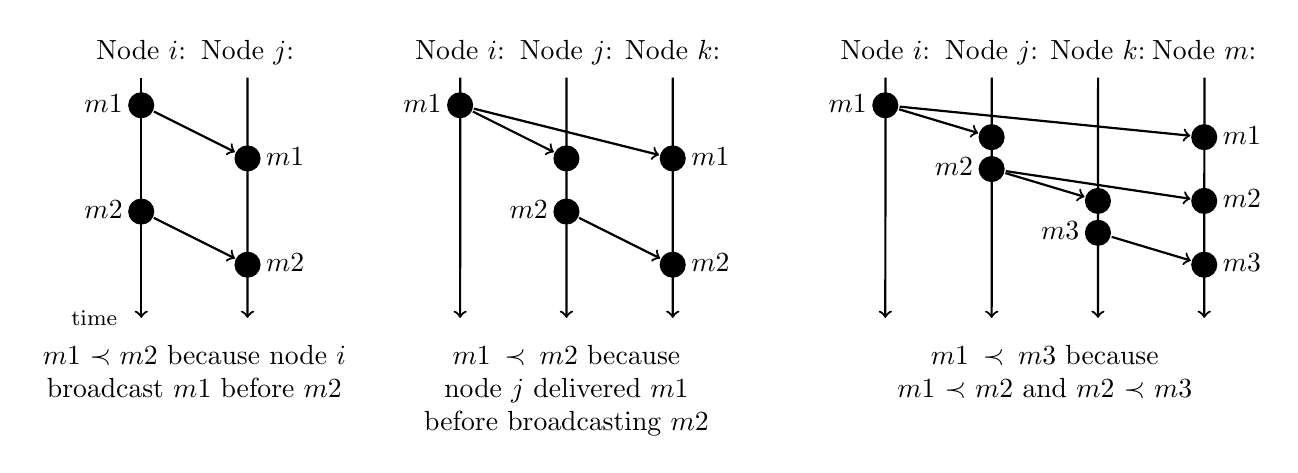
\begin{tikzpicture}[auto,scale=1.35]

\tikzstyle{event}=[circle,fill,minimum size=2pt]
\tikzstyle{label}=[text height=8pt,text depth=3pt]
\tikzstyle{leftlabel}=[label,left=3pt]
\tikzstyle{rightlabel}=[label,right=3pt]
\tikzstyle{every path}=[thick,->]
\tikzstyle{caption}=[text width=4cm,text centered,text height=8pt,below=5pt]

\node [label] (i1name) at (0,2.5) {Node $i$:};
\node [label] (j1name) at (1,2.5) {Node $j$:};
\node [event] (op1send) at (0,2.0) {};
\node [event] (op1recv) at (1,1.5) {};
\node [event] (op2send) at (0,1.0) {};
\node [event] (op2recv) at (1,0.5) {};
\node [leftlabel]  at (0,2.0) {$\isa{m1}$};
\node [rightlabel] at (1,1.5) {$\isa{m1}$};
\node [leftlabel]  at (0,1.0) {$\isa{m2}$};
\node [rightlabel] at (1,0.5) {$\isa{m2}$};
\draw (i1name) -- (0,0) node [left=5pt,at end] {\footnotesize time};
\draw (j1name) -- (1,0);
\draw (op1send) -- (op1recv);
\draw (op2send) -- (op2recv);
\node [caption] at (0.5,0) {
    $\isa{m1} \prec \isa{m2}$
    because node $i$ broadcast $\isa{m1}$ before $\isa{m2}$
};

\node [label] (i2name) at (3,2.5) {Node $i$:};
\node [label] (j2name) at (4,2.5) {Node $j$:};
\node [label] (k2name) at (5,2.5) {Node $k$:};
\node [event] (op3send) at (3,2.0) {};
\node [event] (op3recj) at (4,1.5) {};
\node [event] (op3reck) at (5,1.5) {};
\node [event] (op4send) at (4,1.0) {};
\node [event] (op4reck) at (5,0.5) {};
\node [leftlabel]  at (3,2.0) {$\isa{m1}$};
\node [rightlabel] at (5,1.5) {$\isa{m1}$};
\node [leftlabel]  at (4,1.0) {$\isa{m2}$};
\node [rightlabel] at (5,0.5) {$\isa{m2}$};
\draw (i2name) -- (3,0);
\draw (j2name) -- (4,0);
\draw (k2name) -- (5,0);
\draw (op3send) -- (op3recj);
\draw (op3send) -- (op3reck);
\draw (op4send) -- (op4reck);
\node [caption] at (4.0,0) {
    $\isa{m1} \prec \isa{m2}$
    because node $j$ delivered $\isa{m1}$ before broadcasting $\isa{m2}$
};

\node [label] (i3name) at  (7,2.5) {Node $i$:};
\node [label] (j3name) at  (8,2.5) {Node $j$:};
\node [label] (k3name) at  (9,2.5) {Node $k$:};
\node [label] (m3name) at (10,2.5) {Node $m$:};
\node [event] (op5send) at  (7,2.0) {};
\node [event] (op5recj) at  (8,1.7) {};
\node [event] (op5recm) at (10,1.7) {};
\node [event] (op6send) at  (8,1.4) {};
\node [event] (op6reck) at  (9,1.1) {};
\node [event] (op6recm) at (10,1.1) {};
\node [event] (op7send) at  (9,0.8) {};
\node [event] (op7recm) at (10,0.5) {};
\node [leftlabel]  at  (7,2.0) {$\isa{m1}$};
\node [rightlabel] at (10,1.7) {$\isa{m1}$};
\node [leftlabel]  at  (8,1.4) {$\isa{m2}$};
\node [rightlabel] at (10,1.1) {$\isa{m2}$};
\node [leftlabel]  at  (9,0.8) {$\isa{m3}$};
\node [rightlabel] at (10,0.5) {$\isa{m3}$};
\draw (i3name) -- (7,0);
\draw (j3name) -- (8,0);
\draw (k3name) -- (9,0);
\draw (m3name) -- (10,0);
\draw (op5send) -- (op5recj);
\draw (op5send) -- (op5recm);
\draw (op6send) -- (op6reck);
\draw (op6send) -- (op6recm);
\draw (op7send) -- (op7recm);
\node [caption] at (8.5,0) {
    $\isa{m1} \prec \isa{m3}$ because
    $\isa{m1} \prec \isa{m2}$ and
    $\isa{m2} \prec \isa{m3}$
};

\end{tikzpicture}

\caption{Illustrating the happens-before relation}\label{fig.happens-before}
\end{figure}

Figure~\ref{fig.happens-before} illustrates these three cases, and the formalisation of this
definition appears in Section~\ref{sect.network}.

In practice, the happens-before relationship can be captured using vector timestamps
\cite{Schwarz:1994gl,Fidge:1988tv,Raynal:1996jl}, which are used to implement protocols for causally
ordered delivery \cite{Cachin:2011wt}. As these protocols are widely known and well understood, we
leave them out of scope for this paper.


% Total order broadcast ensures that when nodes broadcast a set of messages to other nodes on the
% network, they are delivered in the same order to all recipients. By contrast, causal ordering is a
% weaker guarantee that allows greater concurrency and thus greater nondeterminism in the network.
% However, it has the advantage that it makes no assumptions about the number of nodes that are
% online.

% TODO happens-before


% There are two families of algorithms for collaborative editing: \emph{operational transformation}
% (OT)~\cite{Ellis:1989ue,Ressel:1996wx,Oster:2006tr,Sun:1998vf,Sun:1998un,Suleiman:1998eu,Nichols:1995fd}
% and \emph{conflict-free replicated datatypes}
% (CRDTs)~\cite{Shapiro:2011wy,Roh:2011dw,Preguica:2009fz,Oster:2006wj,Weiss:2010hx,Nedelec:2013ky,Kleppmann:2016ve}.
% Both allow a document to be modified concurrently on different replicas, with changes applied
% immediately to the local copy, while asynchronously propagating changes to other replicas. The
% goal of these algorithms is to ensure that for all concurrent executions, the replicas converge
% toward the same state without any edits being lost, a property known as \emph{strong eventual
% consistency}~\cite{Shapiro:2011un}.


% CRDTs are a more recent development~\cite{Shapiro:2011un}. While OT is based on transforming
% non-commutative operations so that they have the same effect when reordered, CRDTs define operations
% in a way that makes them commutative by design, making them more amenable to peer-to-peer settings
% in which each node may apply edits in a different order. CRDTs also have attractive performance
% characteristics~\cite{Mehdi:2011ke}.

% TODO Various decentralised algorithms have been proposed and all but one (Oster 2006) have
% subsequently been shown to be incorrect.

\begin{figure}
\centering
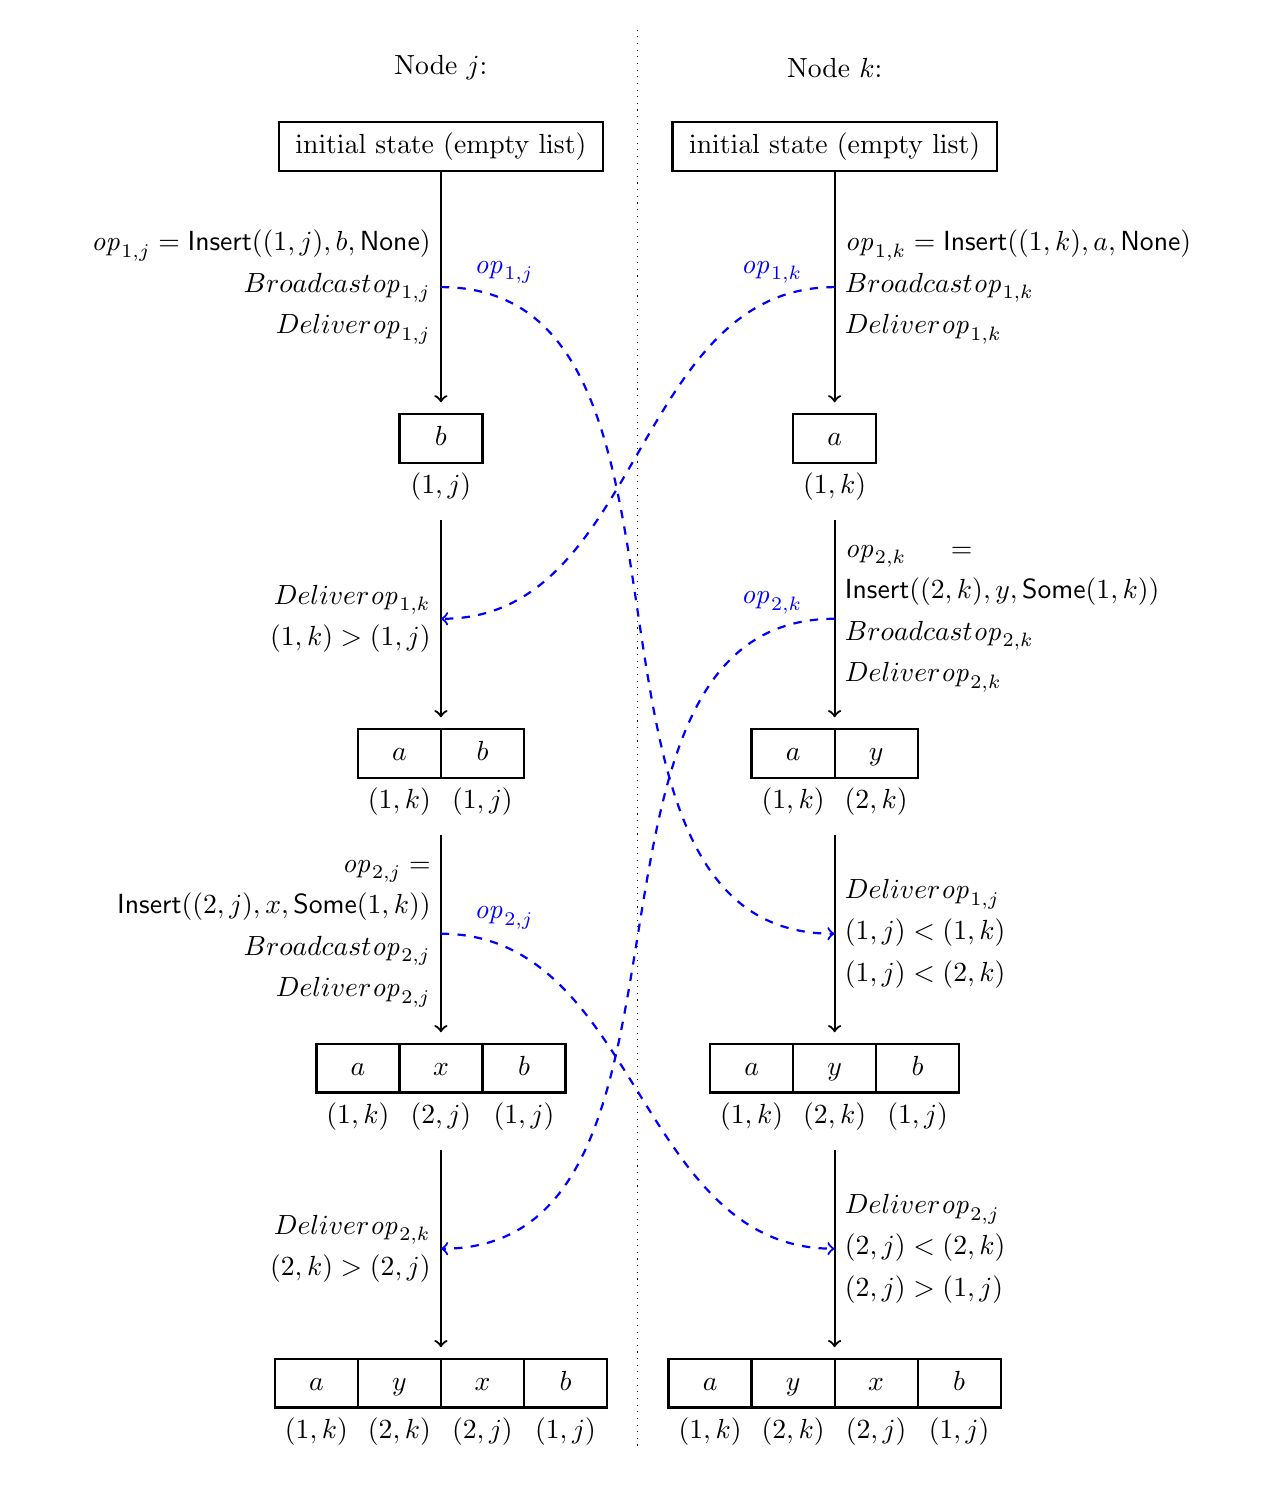
\begin{tikzpicture}[auto,scale=1.0]
\onehalfspacing
\path [draw,dotted] (2.5,-0.5) -- (2.5,17.5);

\tikzstyle{initstate}=[rectangle,draw,inner xsep=6pt,text height=8pt,text depth=3pt]
\tikzstyle{state}=[matrix,column sep={30pt,between origins}]
\tikzstyle{val}=[draw,anchor=base,minimum width=30pt,text height=8pt,text depth=3pt]
\tikzstyle{oid}=[anchor=base]
\tikzstyle{leftevent}=[left,text width=5cm,text ragged left,midway]
\tikzstyle{rightevent}=[right,text width=5cm,text ragged,midway]
\tikzstyle{every path}=[thick,->]

\node (leftR) at (0,17) {Node $j$:};
\node (left1) at (0,16) [initstate] {initial state (empty list)};
\node (left2) at (0,12) [state] {
    \node [val] {$b$};     \\
    \node [oid] {$(1,j)$}; \\
};
\node (left3) at (0,8) [state] {
    \node [val] {$a$};     & \node [val] {$b$};     \\
    \node [oid] {$(1,k)$}; & \node [oid] {$(1,j)$}; \\
};
\node (left4) at (0,4) [state] {
    \node [val] {$a$};     & \node [val] {$x$};     & \node [val] {$b$};     \\
    \node [oid] {$(1,k)$}; & \node [oid] {$(2,j)$}; & \node [oid] {$(1,j)$}; \\
};
\node (left5) at (0,0) [state] {
    \node [val] {$a$};     & \node [val] {$y$};     & \node [val] {$x$};     & \node [val] {$b$};     \\
    \node [oid] {$(1,k)$}; & \node [oid] {$(2,k)$}; & \node [oid] {$(2,j)$}; & \node [oid] {$(1,j)$}; \\
};

\draw (left1) -- (left2) node (send1j) [leftevent] {
    \hfill $\mathit{op}_{1,j} = \mathsf{Insert}((1, j), b, \mathsf{None})$ \\
    \hfill $\text{Broadcast } \mathit{op}_{1,j}$ \\
    \hfill $\text{Deliver } \mathit{op}_{1,j}$ \\
};
\draw (left2) -- (left3) node (recv1k) [leftevent] {
    \hfill $\text{Deliver } \mathit{op}_{1,k}$ \\
    \hfill $(1,k) > (1,j)$ \\
};
\draw (left3) -- (left4) node (send2j) [leftevent] {
    \hfill $\mathit{op}_{2,j} = \mathsf{Insert}((2, j), x, \mathsf{Some}(1,k))$ \\
    \hfill $\text{Broadcast } \mathit{op}_{2,j}$ \\
    \hfill $\text{Deliver } \mathit{op}_{2,j}$ \\
};
\draw (left4) -- (left5) node (recv2k) [leftevent] {
    \hfill $\text{Deliver } \mathit{op}_{2,k}$ \\
    \hfill $(2,k) > (2,j)$ \\
};

\node (rightR) at (5,17) {Node $k$:};
\node (right1) at (5,16) [initstate] {initial state (empty list)};
\node (right2) at (5,12) [state] {
    \node [val] {$a$};     \\
    \node [oid] {$(1,k)$}; \\
};
\node (right3) at (5,8) [state] {
    \node [val] {$a$};     & \node [val] {$y$};     \\
    \node [oid] {$(1,k)$}; & \node [oid] {$(2,k)$}; \\
};
\node (right4) at (5,4) [state] {
    \node [val] {$a$};     & \node [val] {$y$};     & \node [val] {$b$};     \\
    \node [oid] {$(1,k)$}; & \node [oid] {$(2,k)$}; & \node [oid] {$(1,j)$}; \\
};
\node (right5) at (5,0) [state] {
    \node [val] {$a$};     & \node [val] {$y$};     & \node [val] {$x$};     & \node [val] {$b$};     \\
    \node [oid] {$(1,k)$}; & \node [oid] {$(2,k)$}; & \node [oid] {$(2,j)$}; & \node [oid] {$(1,j)$}; \\
};

\draw (right1) -- (right2) node (send1k) [rightevent] {
    $\mathit{op}_{1,k} = \mathsf{Insert}((1, k), a, \mathsf{None})$ \\
    $\text{Broadcast } \mathit{op}_{1,k}$ \\
    $\text{Deliver } \mathit{op}_{1,k}$ \\
};
\draw (right2) -- (right3) node (send2k) [rightevent] {
    $\mathit{op}_{2,k} = \mathsf{Insert}((2, k), y, \mathsf{Some}(1, k))$ \\
    $\text{Broadcast } \mathit{op}_{2,k}$ \\
    $\text{Deliver } \mathit{op}_{2,k}$ \\
};
\draw (right3) -- (right4) node (recv1j) [rightevent] {
    $\text{Deliver } \mathit{op}_{1,j}$ \\
    $(1,j) < (1,k)$ \\
    $(1,j) < (2,k)$ \\
};
\draw (right4) -- (right5) node (recv2j) [rightevent] {
    $\text{Deliver } \mathit{op}_{2,j}$ \\
    $(2,j) < (2,k)$ \\
    $(2,j) > (1,j)$ \\
};

\begin{scope}[dashed,blue]
    \tikzstyle{every node}=[text centered]
    \draw (send1j.east) to [out=0,in=180] (recv1j.west);
    \draw (send2j.east) to [out=0,in=180] (recv2j.west);
    \draw (send1k.west) to [out=180,in=0] (recv1k.east);
    \draw (send2k.west) to [out=180,in=0] (recv2k.east);
    \node at (0.8,14.4) {$\mathit{op}_{1,j}$};
    \node at (0.8, 6.2) {$\mathit{op}_{2,j}$};
    \node at (4.2,14.4) {$\mathit{op}_{1,k}$};
    \node at (4.2,10.2) {$\mathit{op}_{2,k}$};
\end{scope}
\end{tikzpicture}

\caption{RGA example}\label{fig.two-lists}
\end{figure}


%%%%%%%%%%%%%%%%%%%%%%%%%%%%%%%%%%%%%%%%%%%%%%%%%%%%%%%%%%%%%%%%%%%%%%%%%%%%%%%%
% RGA_Network
%%%%%%%%%%%%%%%%%%%%%%%%%%%%%%%%%%%%%%%%%%%%%%%%%%%%%%%%%%%%%%%%%%%%%%%%%%%%%%%%

\section{Conclusion}
\label{sect.conclusion}

\subsection*{Acknowledgements}

\bibliography{references}{}

\end{document}
